\documentclass[default]{beamer}
\setbeamertemplate{navigation symbols}{}

\usetheme{Frankfurt}
%\useoutertheme{infolines}
\usecolortheme{beaver}

\usepackage[utf8]{inputenc}					% Выбор языка и кодировки
\usepackage[english]{babel}	% Языки: русский, английский
\usepackage{csquotes}
\usepackage{tikz}
\usetikzlibrary{arrows,shapes,calc}
\usepackage{animate}
\usepackage{fp}
\usepackage{textpos}
\usepackage{amsfonts}

\usepackage[
	language=auto,
	autolang=other,
	backend=biber,
	style=authortitle,
	sorting=ydnt,
	maxbibnames=5
]{biblatex}
\addbibresource{strl_cai16.bib}
				
\DeclareSourcemap{
	\maps[datatype=bibtex, overwrite]{
		\map{
			\step[fieldset=langid, fieldvalue=english]
			\step[fieldset=doi, null]
			\step[fieldset=issn, null]
			\step[fieldset=isbn, null]
			\step[fieldset=url, null]
			\step[fieldsource=language, fieldset=langid, origfieldval]
		}
	}
}
\DeclareBibliographyDriver{std}{%
	\usebibmacro{bibindex}%
	\usebibmacro{begentry}%
	\usebibmacro{author/editor+others/translator+others}%
	\setunit{\labelnamepunct}\newblock
	\usebibmacro{title}%
	\newunit\newblock
	\usebibmacro{maintitle+booktitle}
	\newunit\newblock
	\usebibmacro{journal}%
	\newunit\newblock
	\usebibmacro{date}%
	\newunit\newblock
	\usebibmacro{finentry}
}
\DeclareBibliographyAlias{article}{std}
\DeclareBibliographyAlias{book}{std}
\DeclareBibliographyAlias{inproceedings}{std}
\DeclareBibliographyAlias{incollection}{std}


\makeatletter
\setbeamertemplate{footline}
{
	\leavevmode%
	\hbox{%
		\begin{beamercolorbox}[wd=.333333\paperwidth,ht=2.25ex,dp=1ex,center]{author
				in head/foot}%
			\usebeamerfont{author in
				head/foot}\insertshortauthor~~\beamer@ifempty{\insertshortinstitute}{}{(\insertshortinstitute)}
		\end{beamercolorbox}%
		\begin{beamercolorbox}[wd=.333333\paperwidth,ht=2.25ex,dp=1ex,center]{title in
				head/foot}%
			\usebeamerfont{title in head/foot}\insertshorttitle
		\end{beamercolorbox}%
		\begin{beamercolorbox}[wd=.333333\paperwidth,ht=2.25ex,dp=1ex,right]{date in
				head/foot}%
			\usebeamerfont{date in head/foot}\insertshortdate{}\hspace*{2em}
			\insertframenumber{}\hspace*{2ex} 
		\end{beamercolorbox}
	}%
	\vskip0pt%
}

\renewcommand*{\bibfont}{\tiny}
\setlength\bibitemsep{-5pt}

\begin{document}
	
	\title[Introduction to AI]{Introduction to Artificial Intelligence: Methods, Models, Algorithms}
	\author[Panov]{\textbf{Aleksandr I. Panov and Konstantin S. Yakovlev}}
	\institute[HSE]{National Research University Higher School of Economics}
	\date{25 July 2017 -- Summer University} 
	
	{
	\setbeamertemplate{headline}{}
	\begin{frame}
		
		\titlepage
		\centering
		\href{mailto:apanov@hse.ru}{apanov@hse.ru}
		
		
\includegraphics[width=25pt]{hse.png} \hspace{10pt}
		
\includegraphics[width=100pt]{ras_en.png} \hspace{10pt}
		
\includegraphics[width=80pt]{frccsc.png}
		
	\end{frame}
	}	

	\section{Metric methods}
	\subsection{1.1}
	\begin{frame}
		\frametitle{Nearest-neighbor method}

		\begin{itemize}
			\item It is a task of classification
			\item Data: $X=(x_i, y_i)^l_{i=1}$
			\item Learning process: we just remember the data
		\end{itemize}
	\end{frame}

	\begin{frame}
		\frametitle{Nearest-neighbor method}
		
		\begin{itemize}
			\item New object $x$
			\item Sorting objects of training data by distance from $x$:
				\[
					\rho(x,x_{(1)})\leq \dots \leq \rho(x, x_{(l)})
				\]
			\item Choose class that is most popular among k nearest neighbors:
			\[
				a(x)=arg\min_{y\in\mathbb Y}\sum_{i=1}^{\textcolor{red}{k}}[y_{(i)}=y]
			\]
				
		\end{itemize}
	\end{frame}

	\begin{frame}
		\frametitle{Nearest-neighbor method}
		
		\centering
		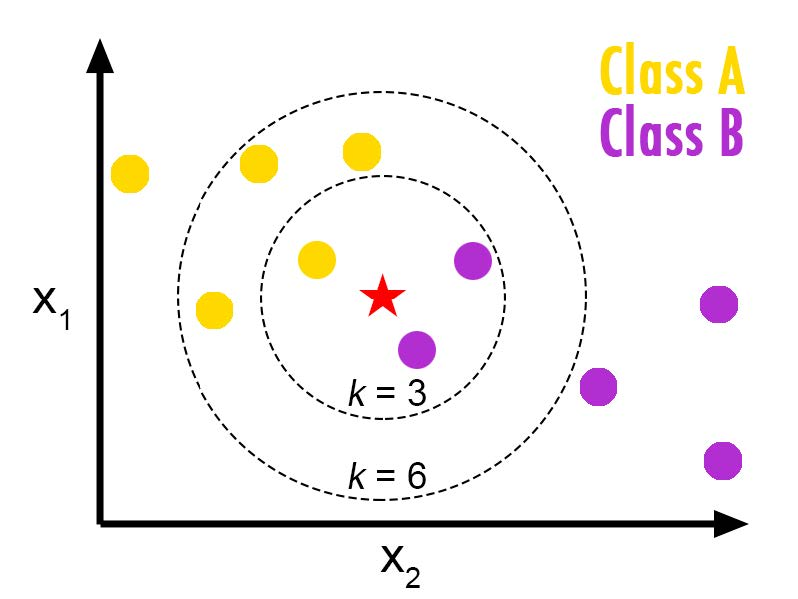
\includegraphics[width=0.8\textwidth]{linear_1.jpg}
	\end{frame}

	\begin{frame}
		\frametitle{Nearest-neighbor method}
		
		\[
			a(x)=arg\min_{y\in\mathbb Y}\sum_{i=1}^{\textcolor{red}{k}}[y_{(i)}=y]
		\]
		
		\begin{itemize}
			\item $k$ - hyperparameter of the algorithm
			\item we can select it via using of hold-out dataset and cross-validation
			\item The larger $k$, the easier the separating surface
		\end{itemize}
	\end{frame}

	\begin{frame}
		\frametitle{How to choose number of neighbors?}
		
		\centering
		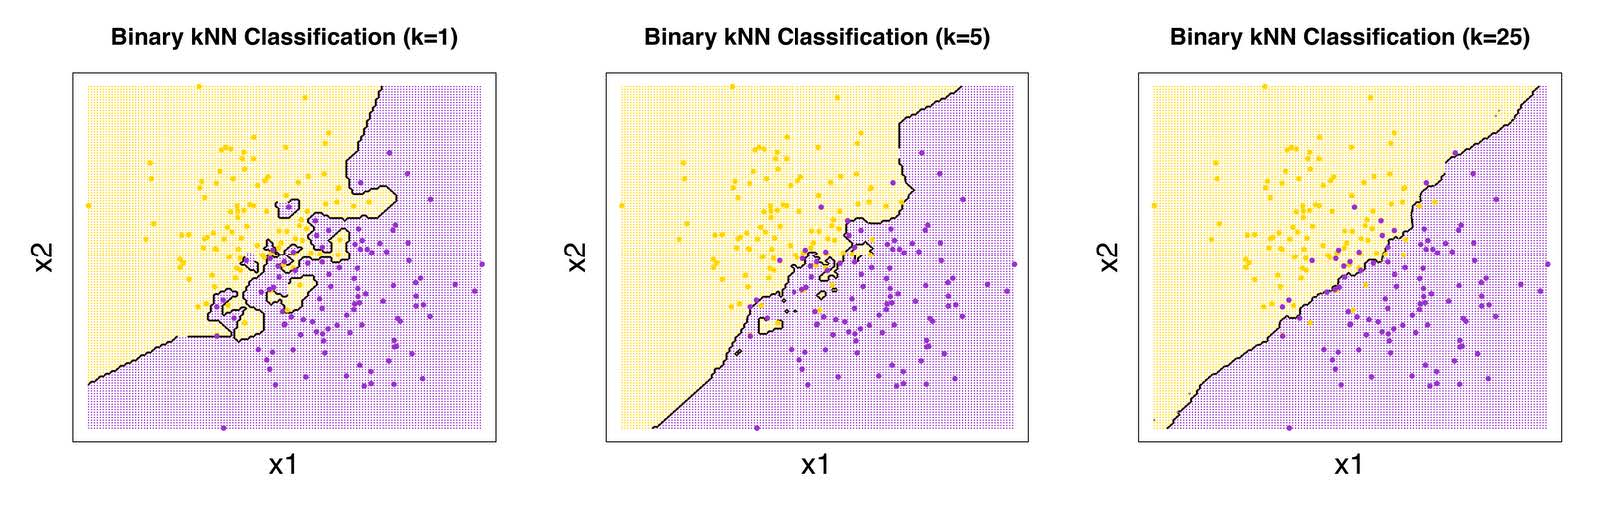
\includegraphics[width=\textwidth]{linear_2.jpg}
	\end{frame}

	\begin{frame}
		\frametitle{How to choose number of neighbors?}
		\begin{itemize}
			\item \textcolor{blue}{Blue} - learning error
			\item \textcolor{red}{Red} - cross-validation error
		\end{itemize}
		\centering
		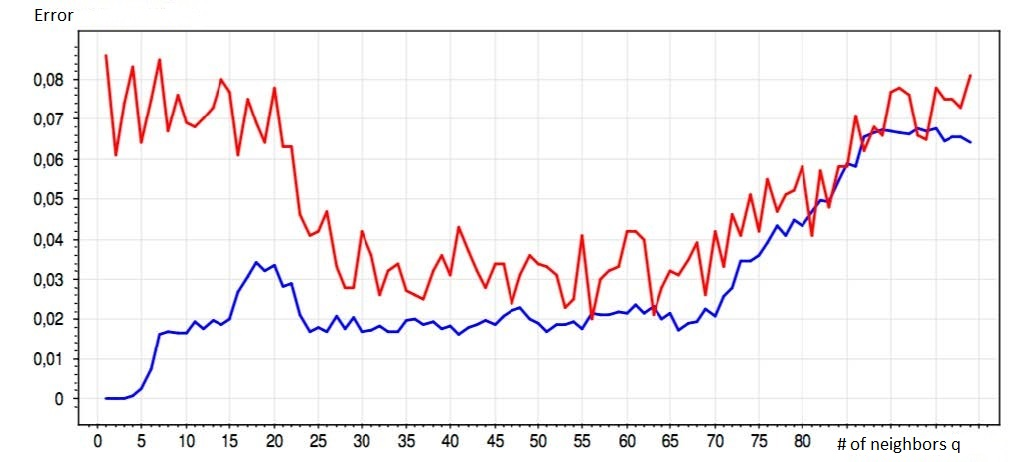
\includegraphics[width=\textwidth]{linear_3.jpg}
	\end{frame}

	\begin{frame}
		\frametitle{Problem of k-NN}
		
		\centering
		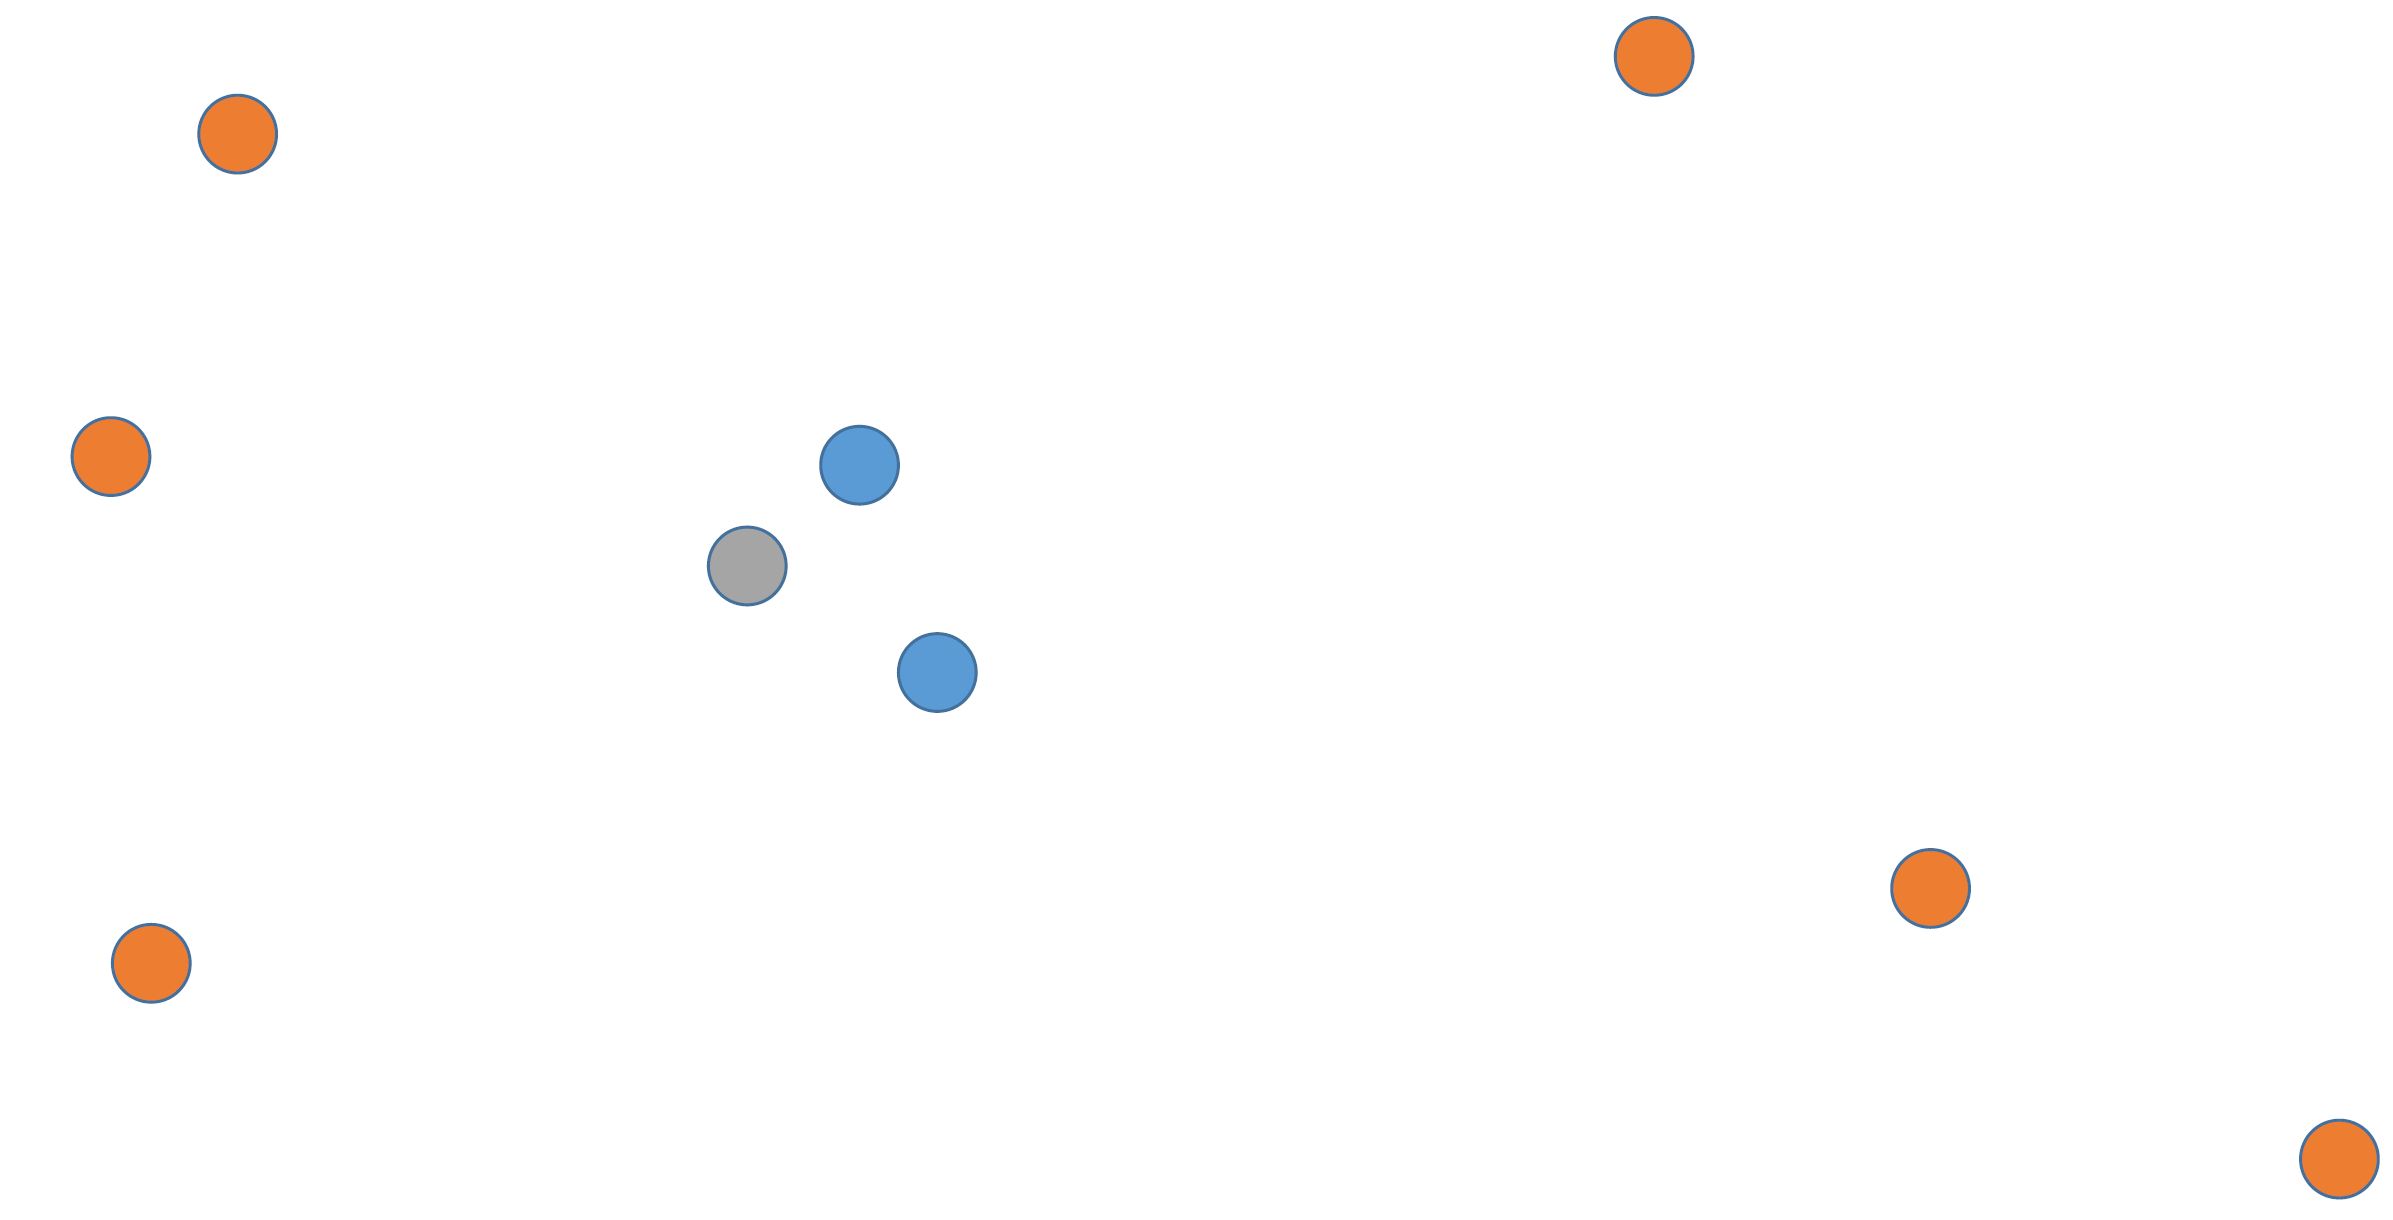
\includegraphics[width=\textwidth]{linear_4.png}
	\end{frame}

	\begin{frame}
		\frametitle{Nearest-neighbor method}
		\Large
		\begin{itemize}
			\item Do not take into account the distances to $k$ nearest neighbors
			\item Closer neighbors should be more important
		\end{itemize}
	\end{frame}

	\begin{frame}
		\frametitle{k-NN with weights}
		\[
			a(x)=arg\min_{y\in\mathbb Y}\sum_{i=1}^k\textcolor{red}{w_i}[y_{(i)}=y]
		\]
		
		Options:
		\begin{itemize}
			\item $w_i=\frac{k+1-1}{k}$
			\item $w_i=q^i$
			\item Not a distance weight
		\end{itemize}
	\end{frame}

	\begin{frame}
		\frametitle{k-NN with weights}
		\[
		a(x)=arg\min_{y\in\mathbb Y}\sum_{i=1}^k\textcolor{red}{w_i}[y_{(i)}=y]
		\]
		
		The Parzenov window:
		\begin{columns}
			\begin{column}{0.5\textwidth}
				\begin{itemize}
					\item $w_i=K(\frac{\rho(x,x_{(i)})}{h})$
					\item $K$ - kernel
					\item $h$ - width of the window
				\end{itemize}
				
			\end{column}
			\begin{column}{0.5\textwidth}
				\centering
				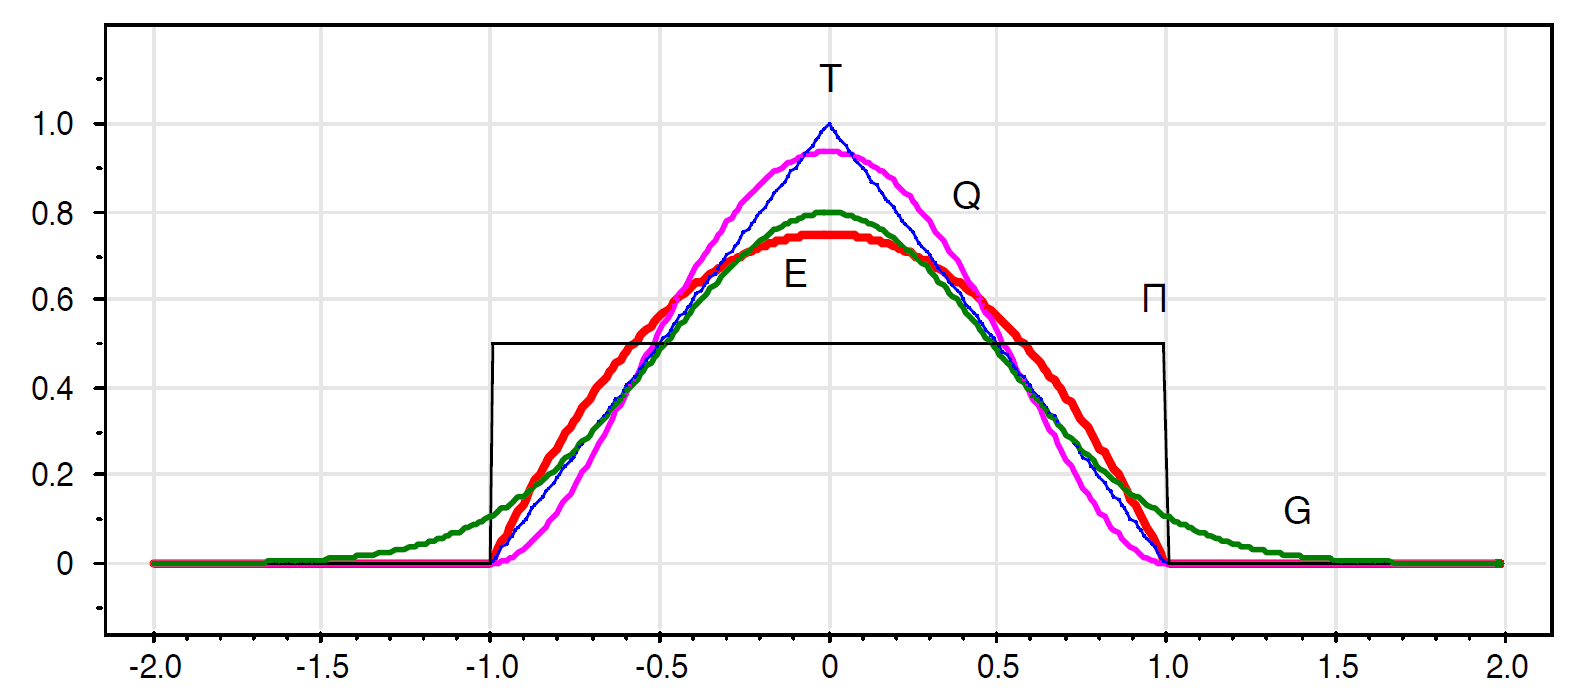
\includegraphics[width=\textwidth]{linear_5.png}
			\end{column}
		\end{columns}
	\end{frame}

	\begin{frame}
		\frametitle{Nearest-neighbor method}
		\begin{itemize}
			\item Gaussian kernel: $K(z)=(2\pi)^{-0.5}\exp^{-\frac{1}{2}z}$
			\item And many others
		\end{itemize}
		\centering
		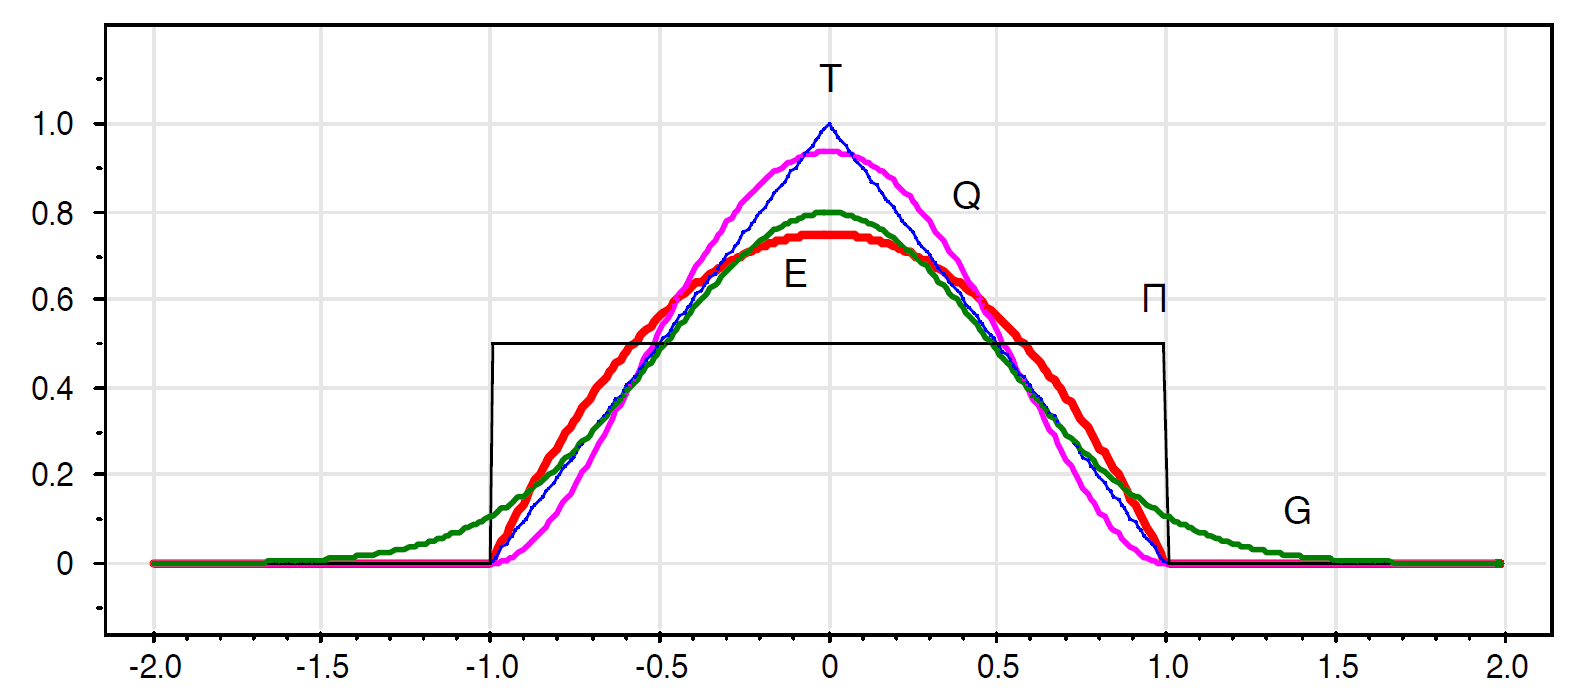
\includegraphics[width=\textwidth]{linear_5.png}
	\end{frame}


	\begin{frame}
		\frametitle{Kernels}
		
		\centering
		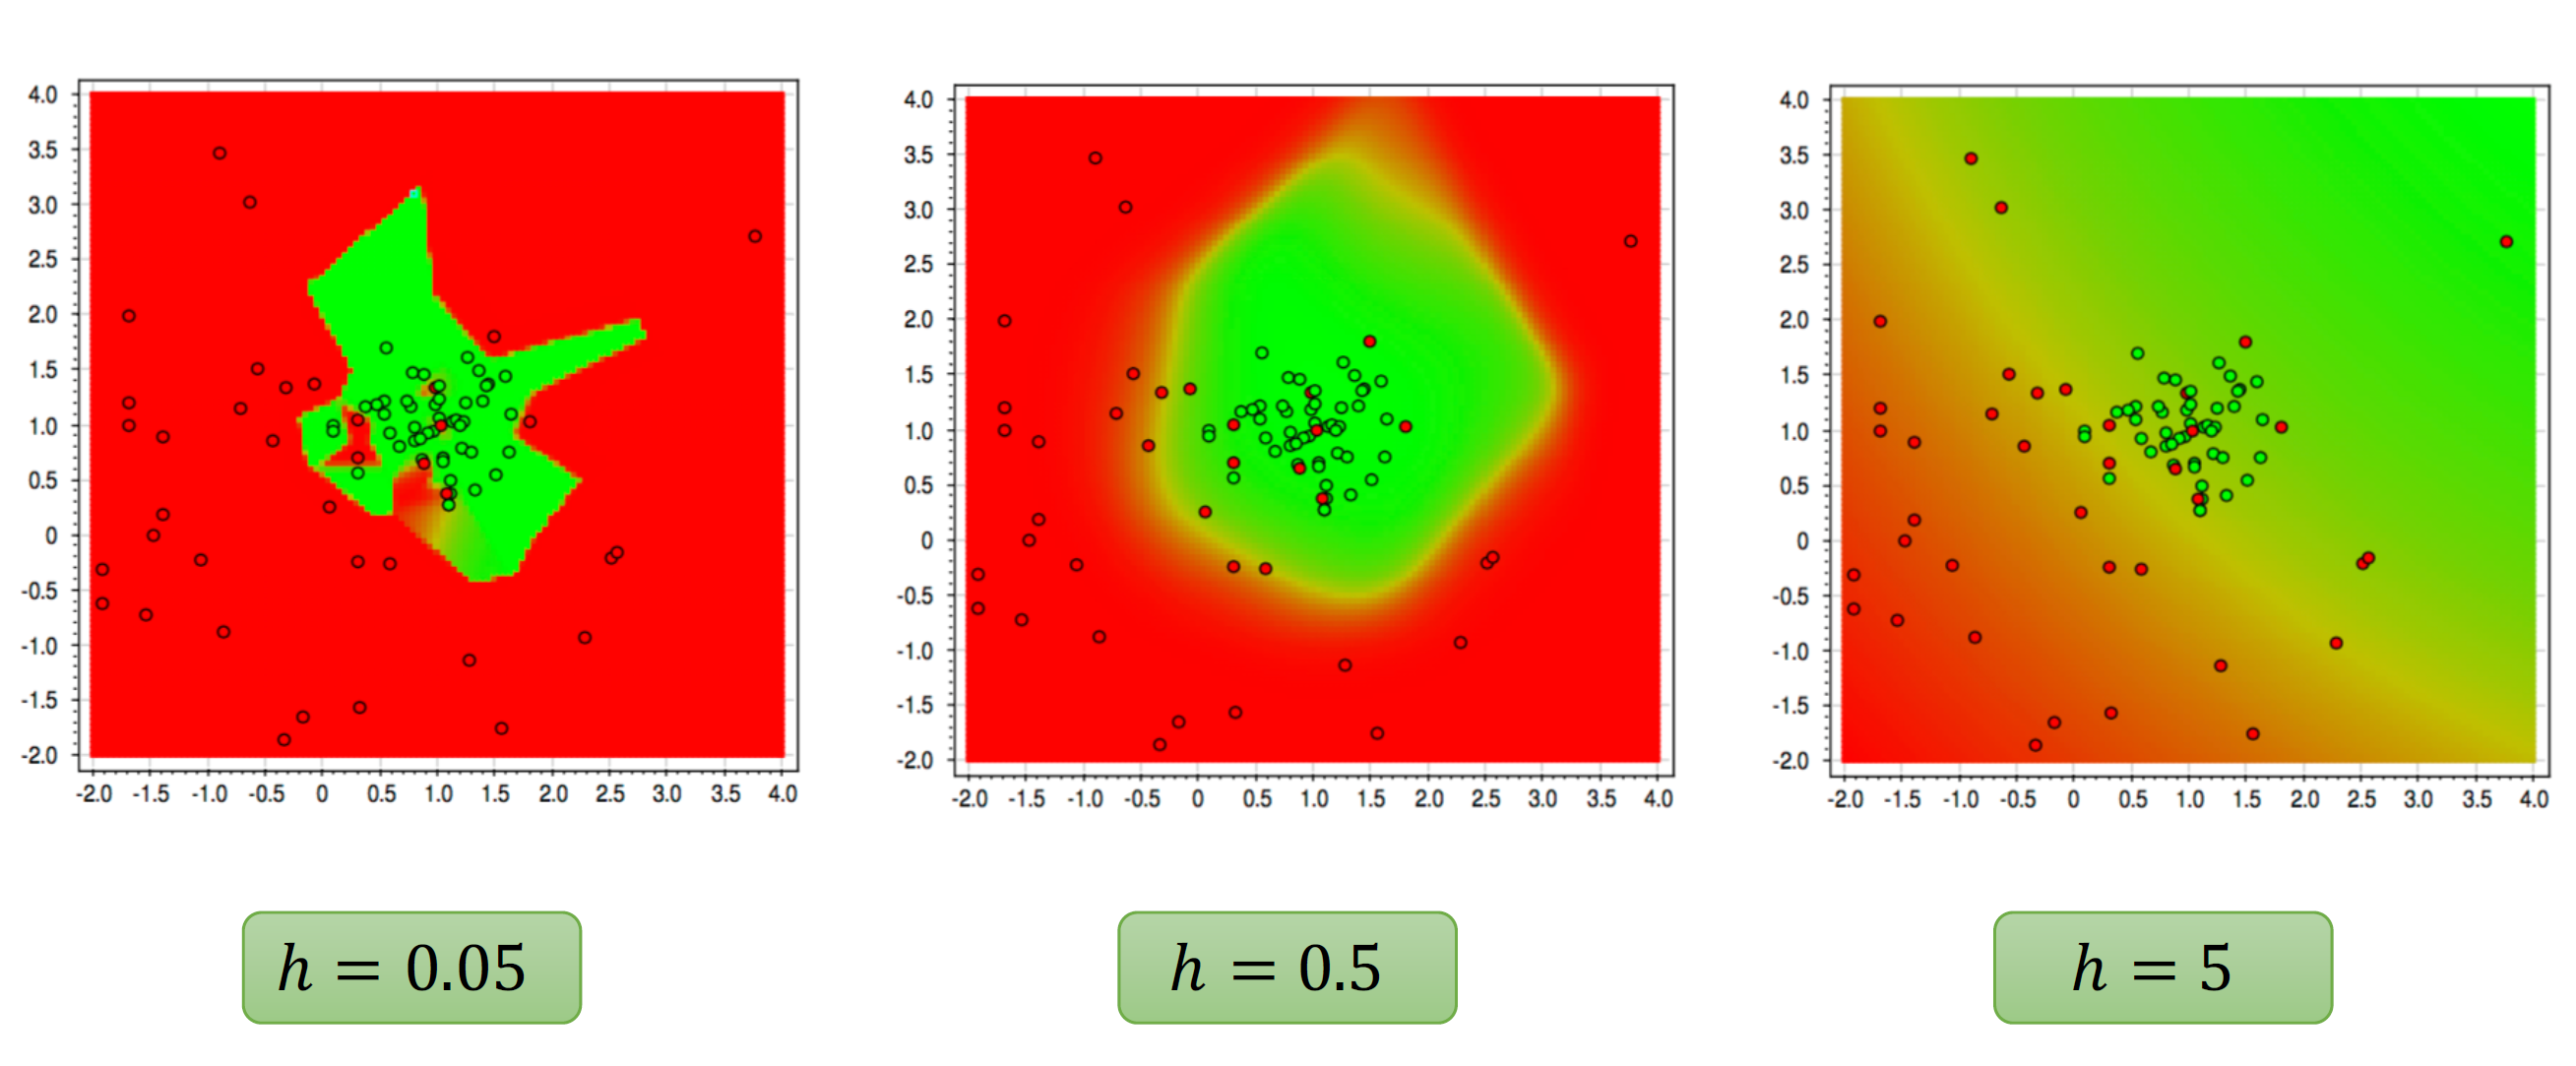
\includegraphics[width=\textwidth]{linear_6.png}
	\end{frame}

	\begin{frame}
		\frametitle{Properties of kNN}
		
		\begin{itemize}
			\item Training is absent - it is only necessary to memorize the training sample
			\item To apply the model, you need to calculate the distances from the new object to all the training objects
			\item Application requires $l\times d$ operations
			\item There are special methods for finding nearest neighbors
		\end{itemize}
	\end{frame}

	\begin{frame}
		\frametitle{kNN for regression}

		\begin{itemize}
			\item Classification:
				\[
				a(x)=arg\min_{y\in\mathbb Y}\sum_{i=1}^{\textcolor{red}{k}}[y_{(i)}=y]
				\]
			\item Regression:
				\[
					a(x)=\frac{\sum_i^k w_iy_{(i)}}{\sum_{i=1}^k w_i}
				\]
		\end{itemize}
	\end{frame}
	\begin{frame}
		\frametitle{kNN for regression}
		
		\begin{itemize}
			\item Gaussian kernel
			\item $h\in\{0.1,1.0,3.0\}$
		\end{itemize}
		\centering
		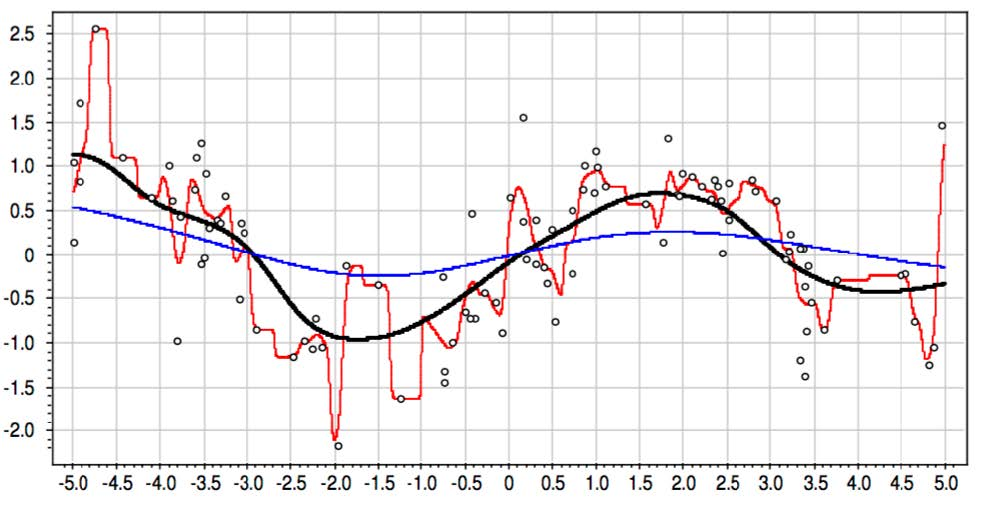
\includegraphics[width=\textwidth]{linear_7.jpg}
	\end{frame}

	\begin{frame}
		\frametitle{kNN for regression}
		
		\begin{itemize}
			\item Rectangle kernel $K(z)=[|z|\leq 1]$
			\item $h\in\{0.1,1.0,3.0\}$
		\end{itemize}
		\centering
		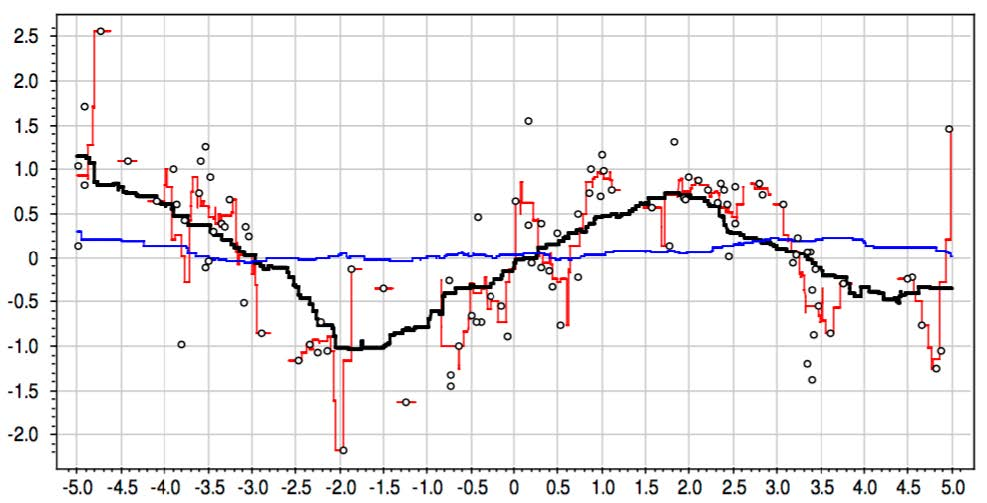
\includegraphics[width=\textwidth]{linear_8.jpg}
	\end{frame}

	\section{Linear regression}
	\subsection{2.1}
	
	\begin{frame}
		\frametitle{One-dimension sample}
		
		\centering
		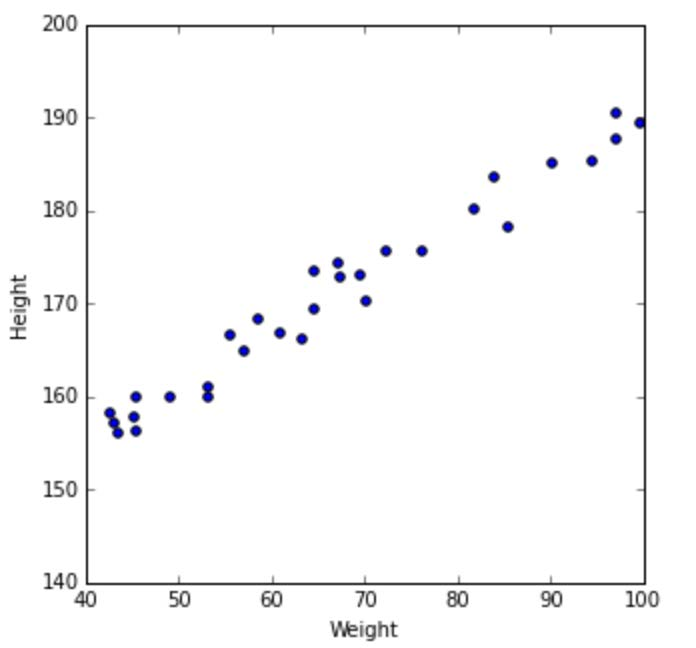
\includegraphics[width=0.8\textwidth]{linear_9.jpg}
	\end{frame}

	\begin{frame}
		\frametitle{One-dimension sample}
		
		\centering
		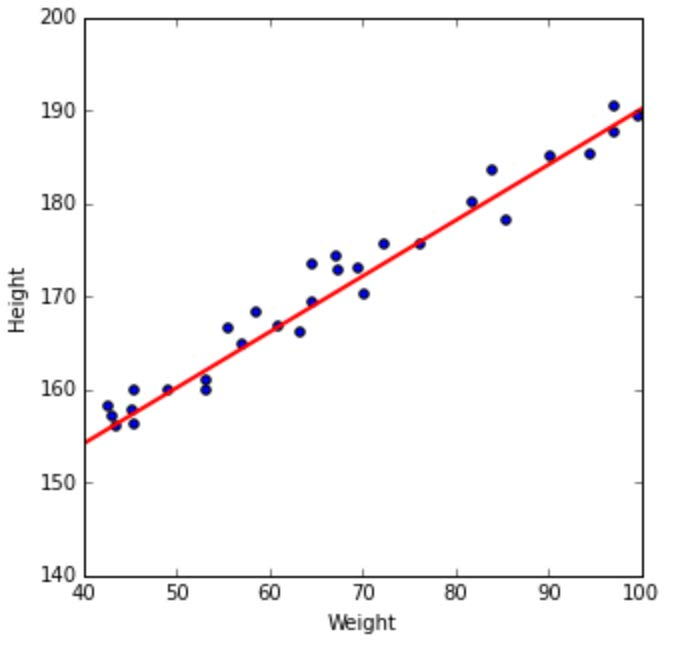
\includegraphics[width=0.8\textwidth]{linear_10.jpg}
	\end{frame}
	
	\begin{frame}
		\frametitle{Paired regression}
		
		\begin{itemize}
			\item The simplest case: only one feature
			\item Model: $a(x)=w_0+w_1x$
			\item Tow parameters: $w_0$ and $w_1$
			\item The simplest model
		\end{itemize}
	\end{frame}

	\begin{frame}
		\frametitle{Linear regression}
		
		\begin{itemize}
			\item Weighted sum of features
			\[
				a(x)=w_0+w_1x^1+\dots + w_dx^d
			\]
			\item $x^1,x^2,\dots,x^d$ - values of features
			\item $w_0,w_1,\dots,w_d$ - parameters
			\item $w_0$ - bias
		\end{itemize}
	\end{frame}

	\begin{frame}
		\frametitle{Linear regression}
		\[
		a(x)=w_0\times 1+w_1x^1+\dots + w_dx^d
		\]
		\begin{itemize}
			\item $w_0$ - as a coefficient with a single feature
			
			\item and if we add it:
		\end{itemize}
	
		\[
			\begin{pmatrix}
			x_{11} & \cdots & x_{1d} & 1\\
			\vdots & & \vdots & \vdots \\
			x_{l1} & \cdots & x_{ld} & 1
			\end{pmatrix}
		\]
	\end{frame}

	\begin{frame}
		\frametitle{Linear regression}
		
		\Large 
		\begin{itemize}
			\item It gives as scalar product
			
			\[
			a(x)=w_0\times 1+w_1x^1+\dots + w_dx^d=\langle w,x\rangle
			\]
			\item Learning:
			\[
			\sum_{i=1}^{l}(\langle w, x_i\rangle-y_i)^2\rightarrow \min_w
			\]
			\item In vector form:
			\[
				Q(w,X)=\frac{1}{q}\|Xw-y\|^2
			\]
		\end{itemize}
	\end{frame}

	\begin{frame}
		\frametitle{Extremes}
		
		\begin{itemize}
			\item Extreme - minimum or maximum
			\item The local minimum is less than all values in some neighborhood
			\item Global minimum - the least of all values
		\end{itemize}
	
		\centering
		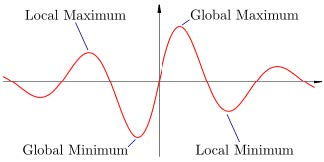
\includegraphics[width=0.6\textwidth]{linear_11.jpg}
	\end{frame}


	\begin{frame}
		\frametitle{Extremes}
		
		\begin{itemize}
			\item Local minima are one of the main problems in machine learning
		\end{itemize}
		
		\centering
		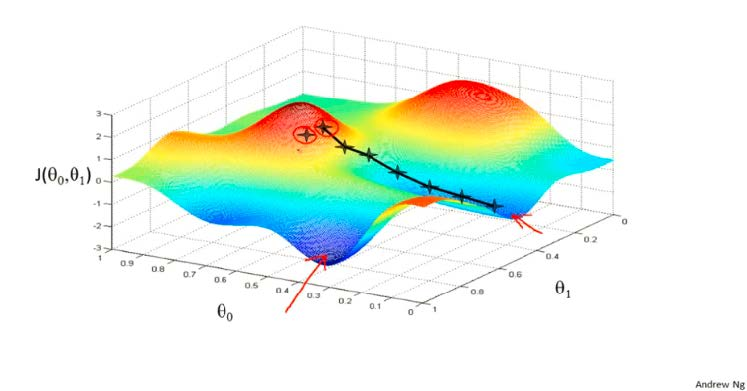
\includegraphics[width=0.8\textwidth]{linear_12.jpg}
	\end{frame}


	\begin{frame}
		\frametitle{The optimality condition}
		
		\begin{itemize}
			\item How do we know if the point $x_0$ is an extremum?
			\item Fermat's theorem: if the point $x_0$ is an extremum, and there is a derivative in it, then $f'(x_0) = 0$
			\item If the function has a derivative everywhere: we need to solve $f'(x) = 0$
			\item If there is a problem with the derivative: no luck
			\item Even if there is a derivative, then what to do with local extremes?
		\end{itemize}
	\end{frame}

	\begin{frame}
		\frametitle{Convex functions}
		
		\begin{itemize}
			\item A convex function if its graph lies below any segment joining two points
		\end{itemize}
		
		\centering
		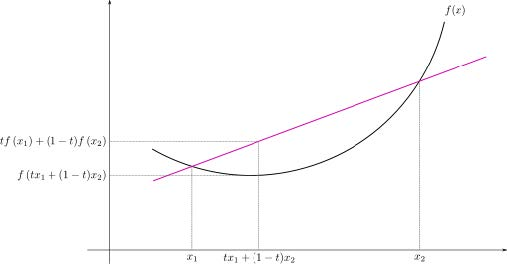
\includegraphics[width=0.8\textwidth]{linear_13.jpg}
	\end{frame}

	\begin{frame}
		\frametitle{Convex functions}
		
		\Large
		\begin{itemize}
			\item The function is convex if, at all points $f''(x)>0$
			\item An important property: any local extremum of a convex function is global
			\item Solving the equation $f'(x)=0$, we obtain global extrema
			\item Conclusion: we will try to choose convex functionals!
		\end{itemize}

	\end{frame}


	\begin{frame}
		\frametitle{An example}
		
		\Large
		\begin{itemize}
			\item Quality functional for linear regression:
			\[
				Q(w_1,\dots,w_d)=\sum_{i=1}^l(w_1x^1+\cdots+w_dx^d-y_i)^2
			\]
			\item How to search for its minimum?
		\end{itemize}
		
	\end{frame}

	\begin{frame}
		\frametitle{Derivative in direction}
		
		\begin{itemize}
			\item How fast is the function growing in a particular direction?
		\end{itemize}
		
		\centering
		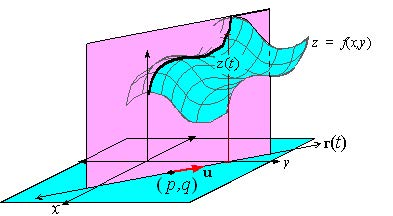
\includegraphics[width=0.8\textwidth]{linear_14.jpg}
	\end{frame}

	\begin{frame}
		\frametitle{Derivative in direction}
		
		\Large
		\begin{itemize}
			\item Direction: $v$ and $\|v\|=1$
			\item Derivative:
			
			\[
				f_v'(x_0)=\lim_{t\rightarrow 0}\frac{f(x_0+tv)-f(x_0)}{t}
			\]
		\end{itemize}
		
	\end{frame}


	\begin{frame}
		\frametitle{Partial derivative}
		
		\begin{itemize}
			\item How fast is the function changing along the variable $x_i$?
			\item The partial derivative with respect to $x_i$:
			\[
				\frac{\partial f}{\partial x_i}=\lim_{t\rightarrow 0}\frac{f(x_1,\dots,x_i+t,\dots,x_d)-f(x_1,\dots,x_i,\dots,x_d)}{t}
			\]
		\end{itemize}
		
		\centering
		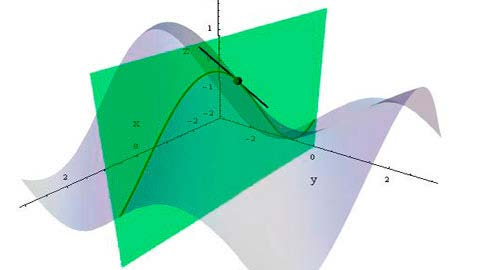
\includegraphics[width=0.6\textwidth]{linear_15.jpg}
	\end{frame}


	\begin{frame}
		\frametitle{Gradient}
		
		\Large
		\begin{itemize}
			\item Gradient is vector of partial derivatives:
			
			\[
			\nabla f(x)=\left(\frac{\partial f}{\partial x_1},\dots,\frac{\partial f}{\partial x_d} \right)
			\]
			\item Gradient has a very important property!
		\end{itemize}
		
	\end{frame}
		
	\begin{frame}
		\frametitle{Gradient}
		
		\Large
		\begin{itemize}
			\item Lets fix a point $x_0$
			\item In which direction is the function growing fastest?
			\[
				f_v'(x_0)\rightarrow \max_v
			\]
			\item Relationship of directional derivative and gradient:
			\[
				f_v'(x_0)=\langle \nabla f (x_0,v)\rangle=\|\nabla f(x_0)\|\times \|v\|\times \cos\phi
			\]
		\end{itemize}
		
	\end{frame}

	\begin{frame}
		\frametitle{Gradient}
		
		\Large
		\begin{itemize}
			\item An arbitrary direction is maximal if the direction coincides with the gradient!
			\item \textbf{Gradient - the direction of the steepest growth of the function}
			\item Antigradient - the direction of steepest descent
		\end{itemize}
		
		\end{frame}


	
	\begin{frame}
		\frametitle{The optimality condition}
		
		\begin{itemize}
			\item How do we know if the point $x_0$ is an extremum?
			\item Fermat's theorem: if the point $x_0$ is an extremum, and there is a gradient in it, then $\nabla f(x_0) = 0$
			\item If the function has a gradient everywhere: we need to solve $\nabla f(x) = 0$
			\item If there is a problem with the gradient: no luck
		\end{itemize}
	\end{frame}

	\begin{frame}
		\frametitle{Extremes}
		
		\begin{itemize}
			\item The problem with local extremes is still relevant
		\end{itemize}
		
		\centering
		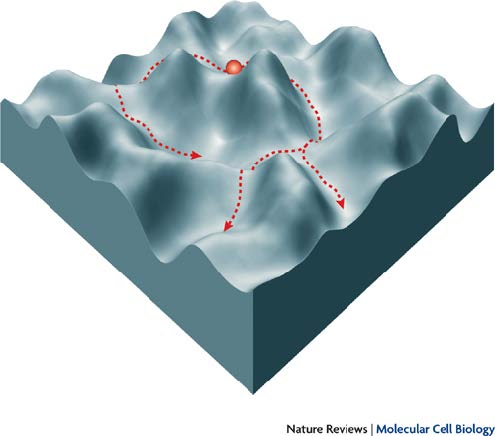
\includegraphics[width=0.6\textwidth]{linear_16.jpg}
	\end{frame}


	\begin{frame}
		\frametitle{Convex functions}
		
		\begin{columns}
			\Large
			\begin{column}{0.5\textwidth}
				The function is convex if its graph lies below the segment joining any two points
			\end{column}
			\begin{column}{0.5\textwidth}
				\centering
				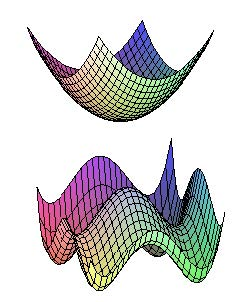
\includegraphics[width=\textwidth]{linear_17.jpg}
			\end{column}
		
		\end{columns}
	
		
	\end{frame}
		

	\section{Learning linear regressors}
	\subsection{3.1}
	
	\begin{frame}
		\frametitle{Optimization problem}
		
		\[
			Q(w,X)=\frac{1}{l}\sum_{i=1}{l}(\langle w,x_i \rangle-y_i)^2-\rightarrow min_w
		\]
		
		\begin{itemize}
			\item A gradient exists at any point
			\item Convex function
			\item The only minimum (not always)
		\end{itemize}
	\end{frame}

	\begin{frame}
		\frametitle{Optimization problem}
		
		\[
		\nabla Q(w, X)=\left(\frac{\partial Q}{\partial w_1},\dots,\frac{\partial Q}{\partial w_d} \right)
		\]
		
		Derivatives:
		\[
			\frac{\partial Q}{\partial w_j}=\frac{2}{l}\sum_{i=1}{l}x_i^j(,\langle w,x_i\rangle-y_i)
		\]
	\end{frame}
	
	
	\begin{frame}
		\frametitle{Learning linear regressor}

		\begin{itemize}
			\item In a vector form:
			\[
				Q(w,X)=\frac{1}{l}\|Xw-y\|^2
			\]
			
			\item Condition of minimum:
			\[
				\nabla Q(w,X)=0
			\]
			\item What if we try to solve this system of equations?
		\end{itemize}
	\end{frame}

	\begin{frame}
		\frametitle{Learning linear regressor}
		
		\begin{itemize}
			\item We can solve it analytically:
			\[
				w=(X^TX)^{-1}X^Ty
			\]
			
			\item But the matrix inversion is a very complicated operation
			\item Gradient descent much faster
		\end{itemize}
	\end{frame}
	
	\section{Optimization methods}
	\subsection{4.1}
	\begin{frame}
		\frametitle{Paired regression}
		
		\begin{itemize}
			\item The simplest case: only one feature
			\item Model: $a(x)=w_0+w_1x$
			\item Tow parameters: $w_0$ and $w_1$
			\item Quality functional: $Q(w_0,w_1)=\sum_{i=1}^l (w_1x_i+w_0-y_i)^2$
		\end{itemize}
		
		\centering
		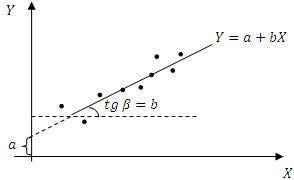
\includegraphics[width=0.5\textwidth]{linear_18.jpg}
	\end{frame}

	\begin{frame}
		\frametitle{Paired regression}
		
		\begin{columns}
			\begin{column}{0.4\textwidth}
				\centering
				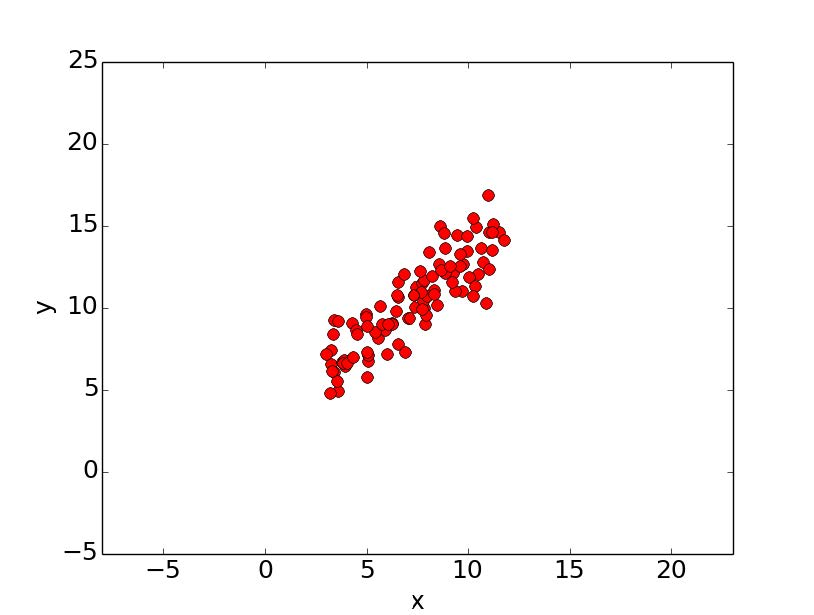
\includegraphics[width=0.9\textwidth]{linear_19.jpg}
				
				\huge
				Sample
			\end{column}
			\begin{column}{0.6\textwidth}
				\centering
				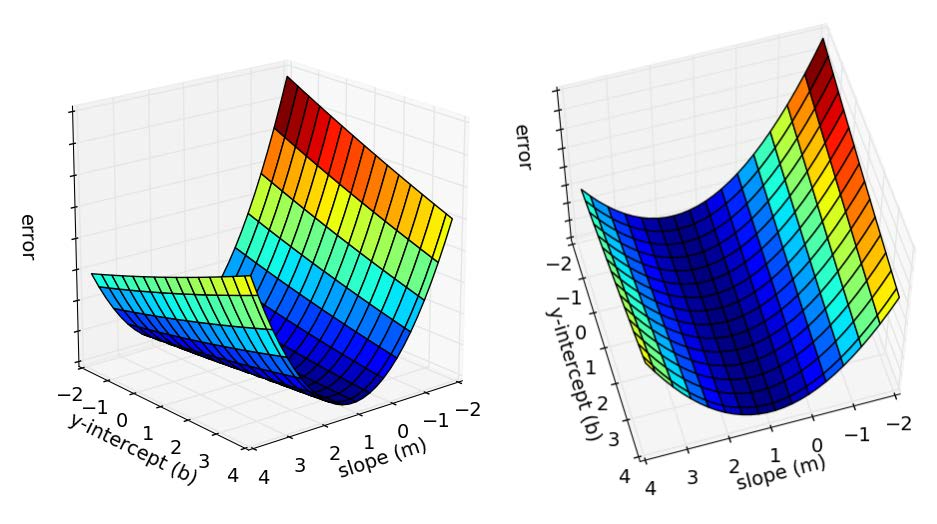
\includegraphics[width=0.9\textwidth]{linear_20.jpg}
				
				\huge
				Quality functional
			\end{column}
		
		\end{columns}
		
	\end{frame}


	\begin{frame}
		\frametitle{Gradient descent}
		
		\begin{columns}
			\begin{column}{0.6\textwidth}
				\begin{itemize}
					\item Suppose we have chosen the initial approximation $w^0=(w_0^0,w_1^0)$
					\item How to improve it?
					\item Stepping towards the steepest descent
					\item That is, towards the anti-gradient!
				\end{itemize}
			\end{column}
			\begin{column}{0.6\textwidth}
				\centering
				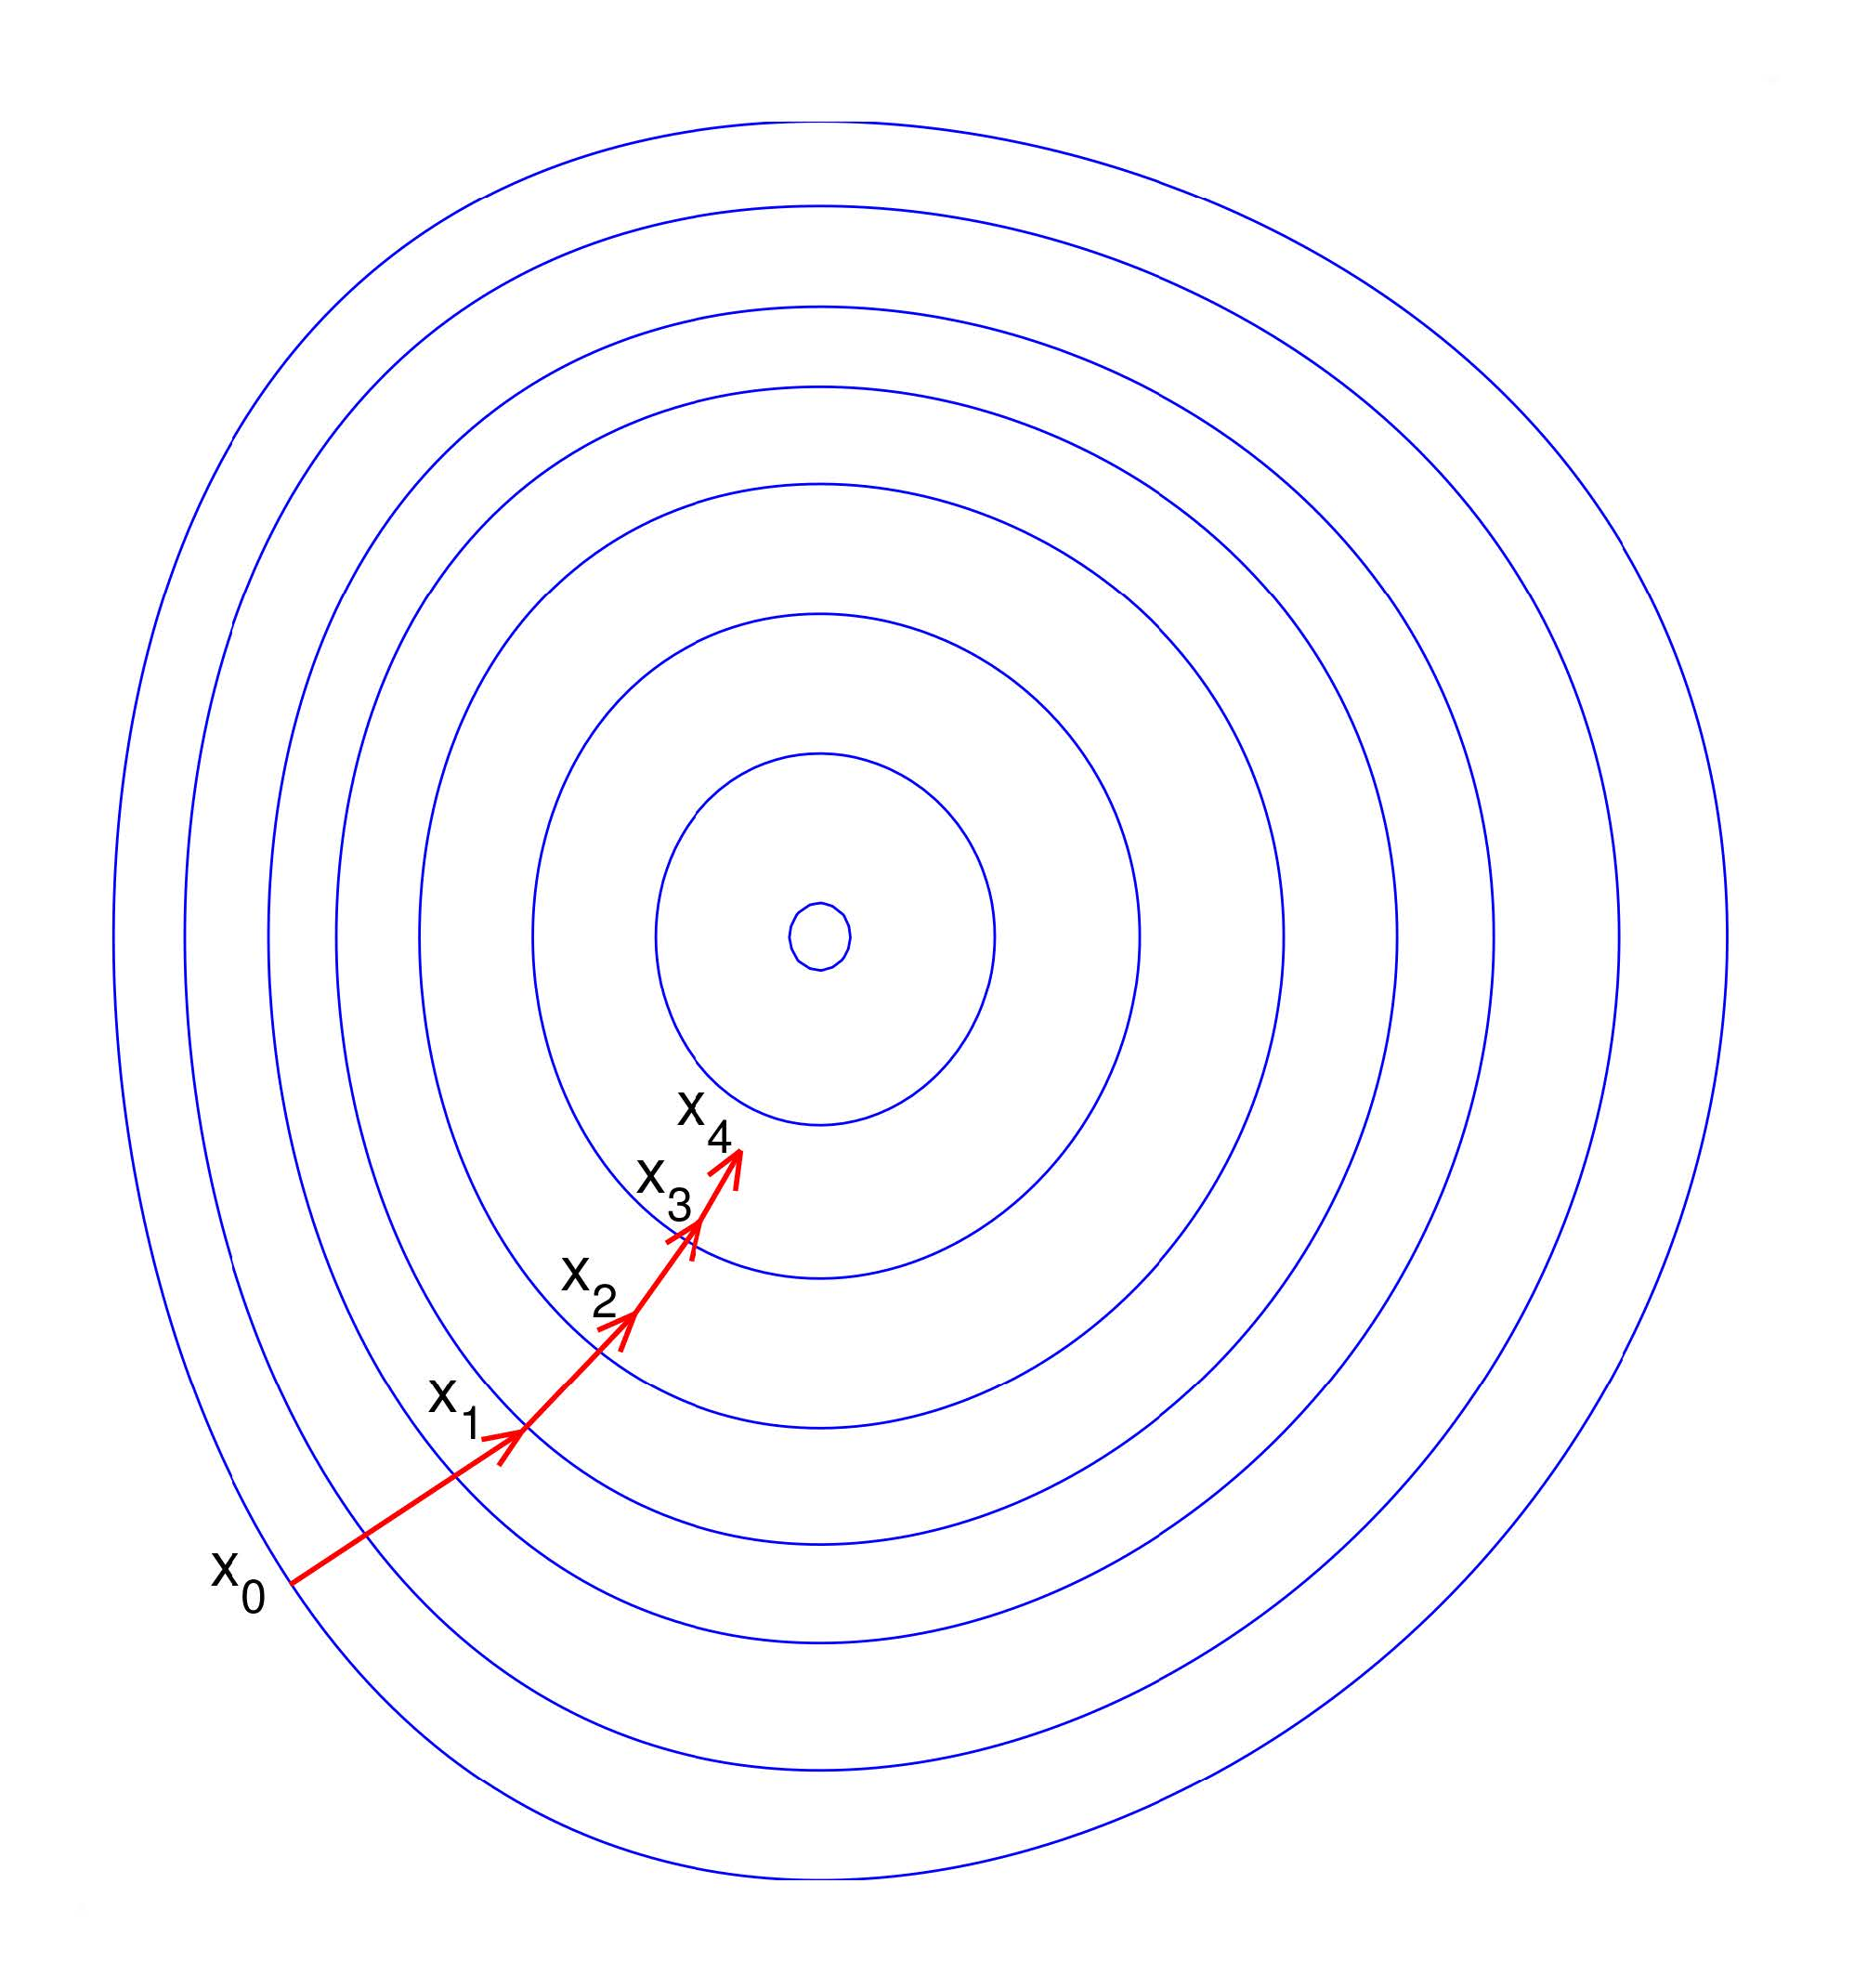
\includegraphics[width=0.9\textwidth]{linear_21.jpg}
			\end{column}
			
		\end{columns}
		
	\end{frame}


	\begin{frame}
		\frametitle{Gradient descent}
		
		\Large
		\begin{itemize}
			\item Repeat until convergence
			
			\[
			w^t=w^{t-1}-\eta \nabla Q(w^{t-1})
			\]
			
			\item convergence: $\|w^t-w^{t-1}<\epsilon\|$
		\end{itemize}
		
	\end{frame}
		

	\begin{frame}
		\frametitle{Gradient for pair regression}
		
		\Large
		\[
			Q(w_0,w_1)=\sum_{i=1}^l (w_1x_i+w_0-y_i)^2
		\]

		Partial derivatives:

			
		\[
		\frac{\partial Q}{\partial w_1}=2\sum_{i=1}^l (w_1x_i+w_0-y_i)x_i
		\]
		
		\[
		\frac{\partial Q}{\partial w_0}=2\sum_{i=1}^l (w_1x_i+w_0-y_i)
		\]
		
	\end{frame}		

	
	\begin{frame}	
		\frametitle{Paired regression}
		
		\centering
		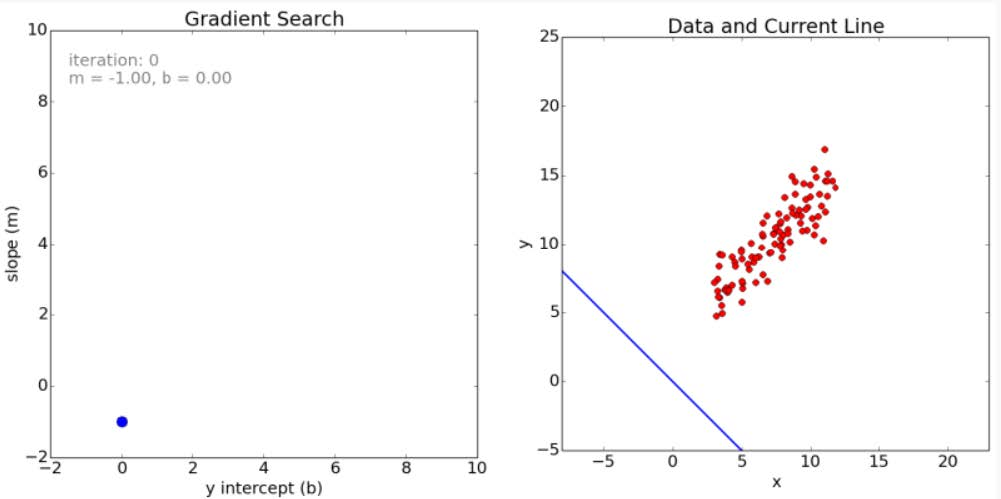
\includegraphics[width=0.8\textwidth]{linear_22.jpg}
	\end{frame}

	\begin{frame}	
\frametitle{Paired regression}

\centering
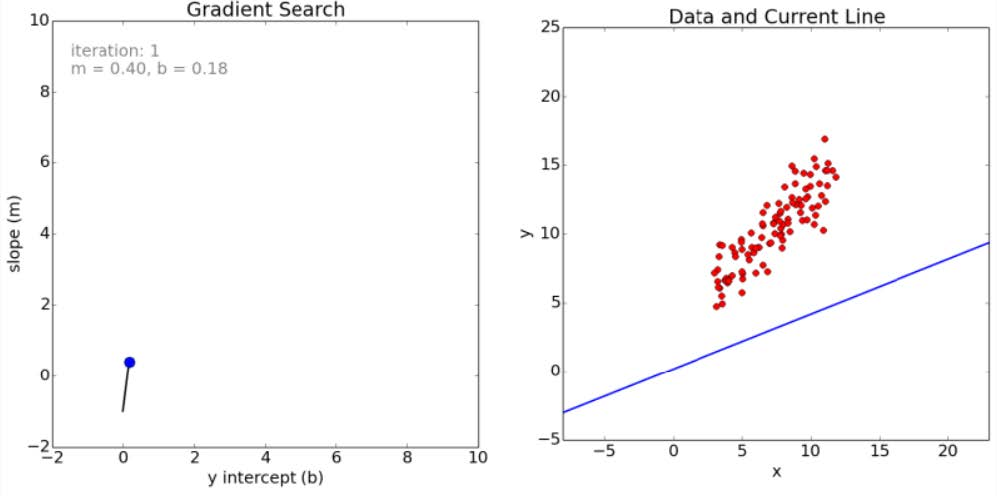
\includegraphics[width=0.8\textwidth]{linear_23.jpg}
\end{frame}

	\begin{frame}	
\frametitle{Paired regression}

\centering
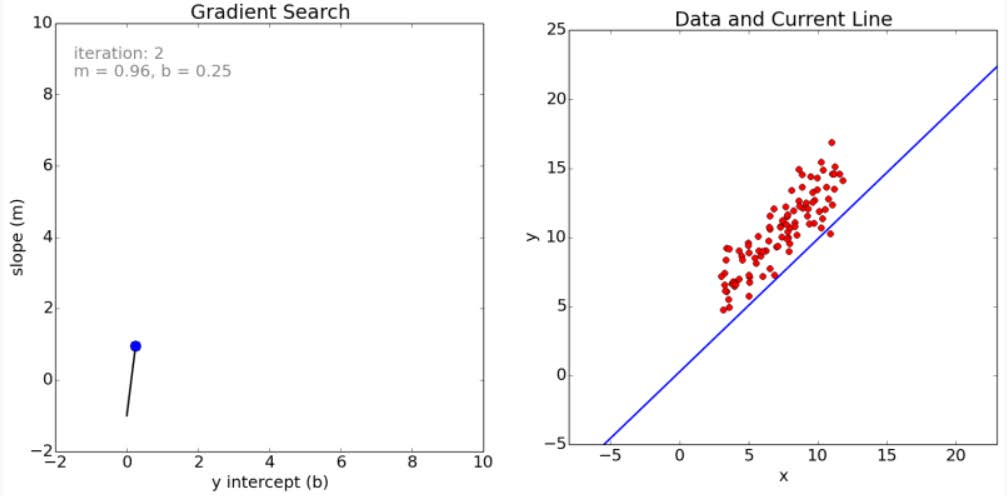
\includegraphics[width=0.8\textwidth]{linear_24.jpg}
\end{frame}

	\begin{frame}	
\frametitle{Paired regression}

\centering
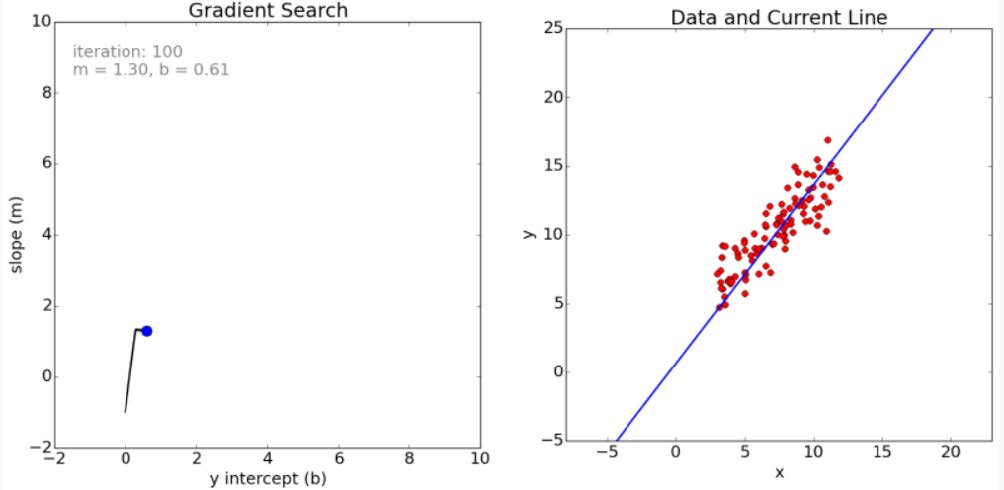
\includegraphics[width=0.8\textwidth]{linear_25.jpg}
\end{frame}

	\begin{frame}	
\frametitle{Paired regression}

\centering
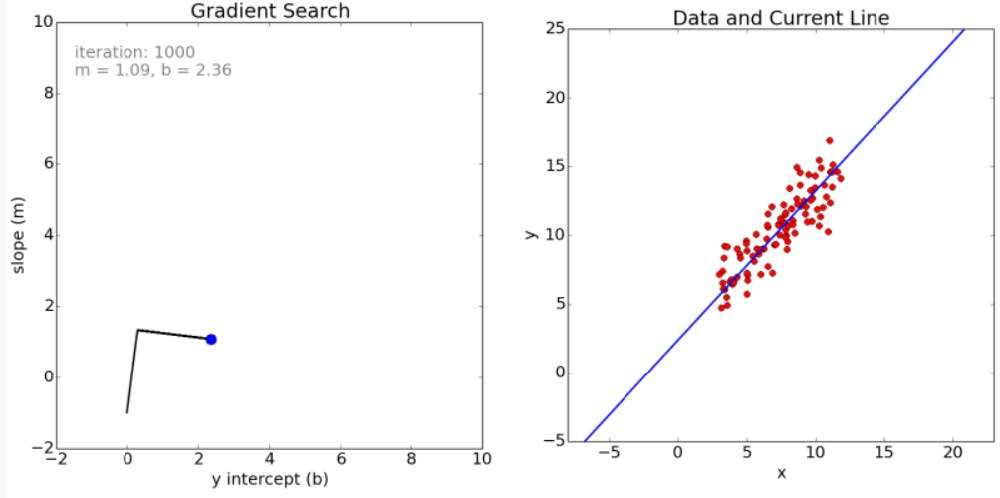
\includegraphics[width=0.8\textwidth]{linear_26.jpg}
\end{frame}

	\begin{frame}	
\frametitle{Paired regression}

\centering
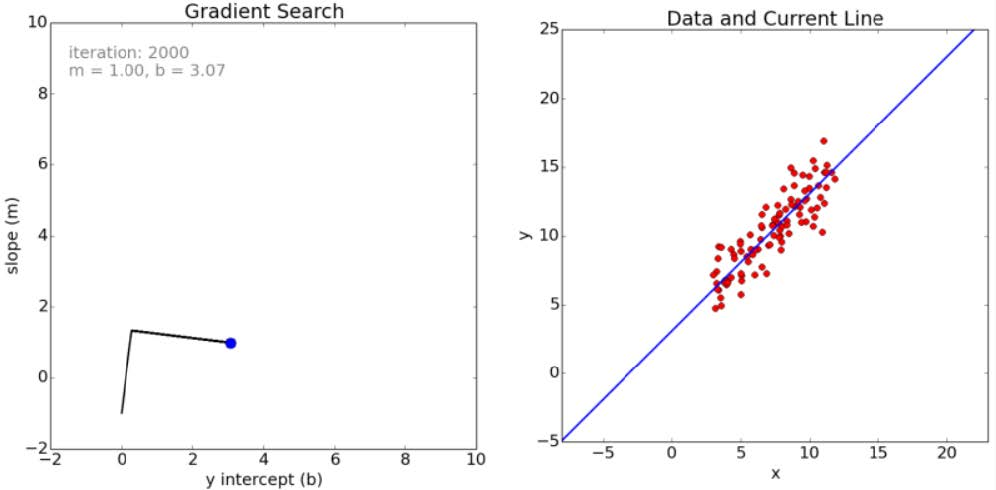
\includegraphics[width=0.8\textwidth]{linear_27.jpg}
\end{frame}

	\begin{frame}	
\frametitle{Paired regression}

\centering
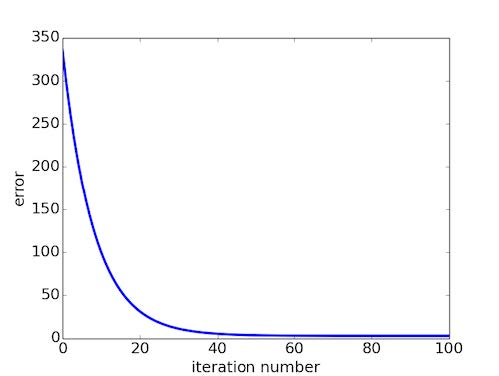
\includegraphics[width=0.8\textwidth]{linear_28.jpg}
\end{frame}

	\begin{frame}	
\frametitle{Local minima}

\Large
Gradient descent can find only local minima

\centering
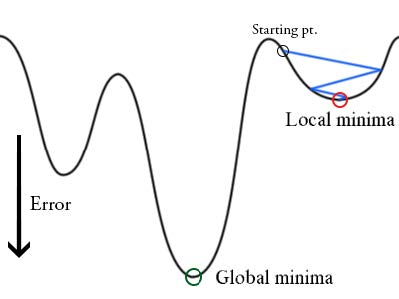
\includegraphics[width=0.6\textwidth]{linear_29.jpg}
\end{frame}

	\begin{frame}	
\frametitle{Local minima}

\Large
\begin{itemize}
	\item The result depends on the initial approximation
	\item Multi-start
	
\end{itemize}

\centering
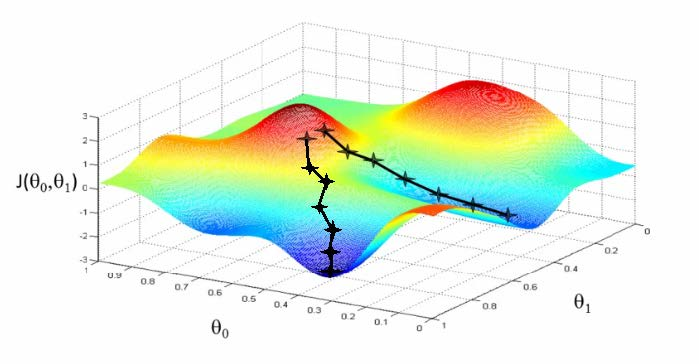
\includegraphics[width=0.8\textwidth]{linear_30.jpg}
\end{frame}

	\begin{frame}	
		\frametitle{Size of step}
		
		\Large
		\begin{itemize}
			\item Choosing of the stepsize  $\eta$ is art
			
		\end{itemize}
		
		\centering
		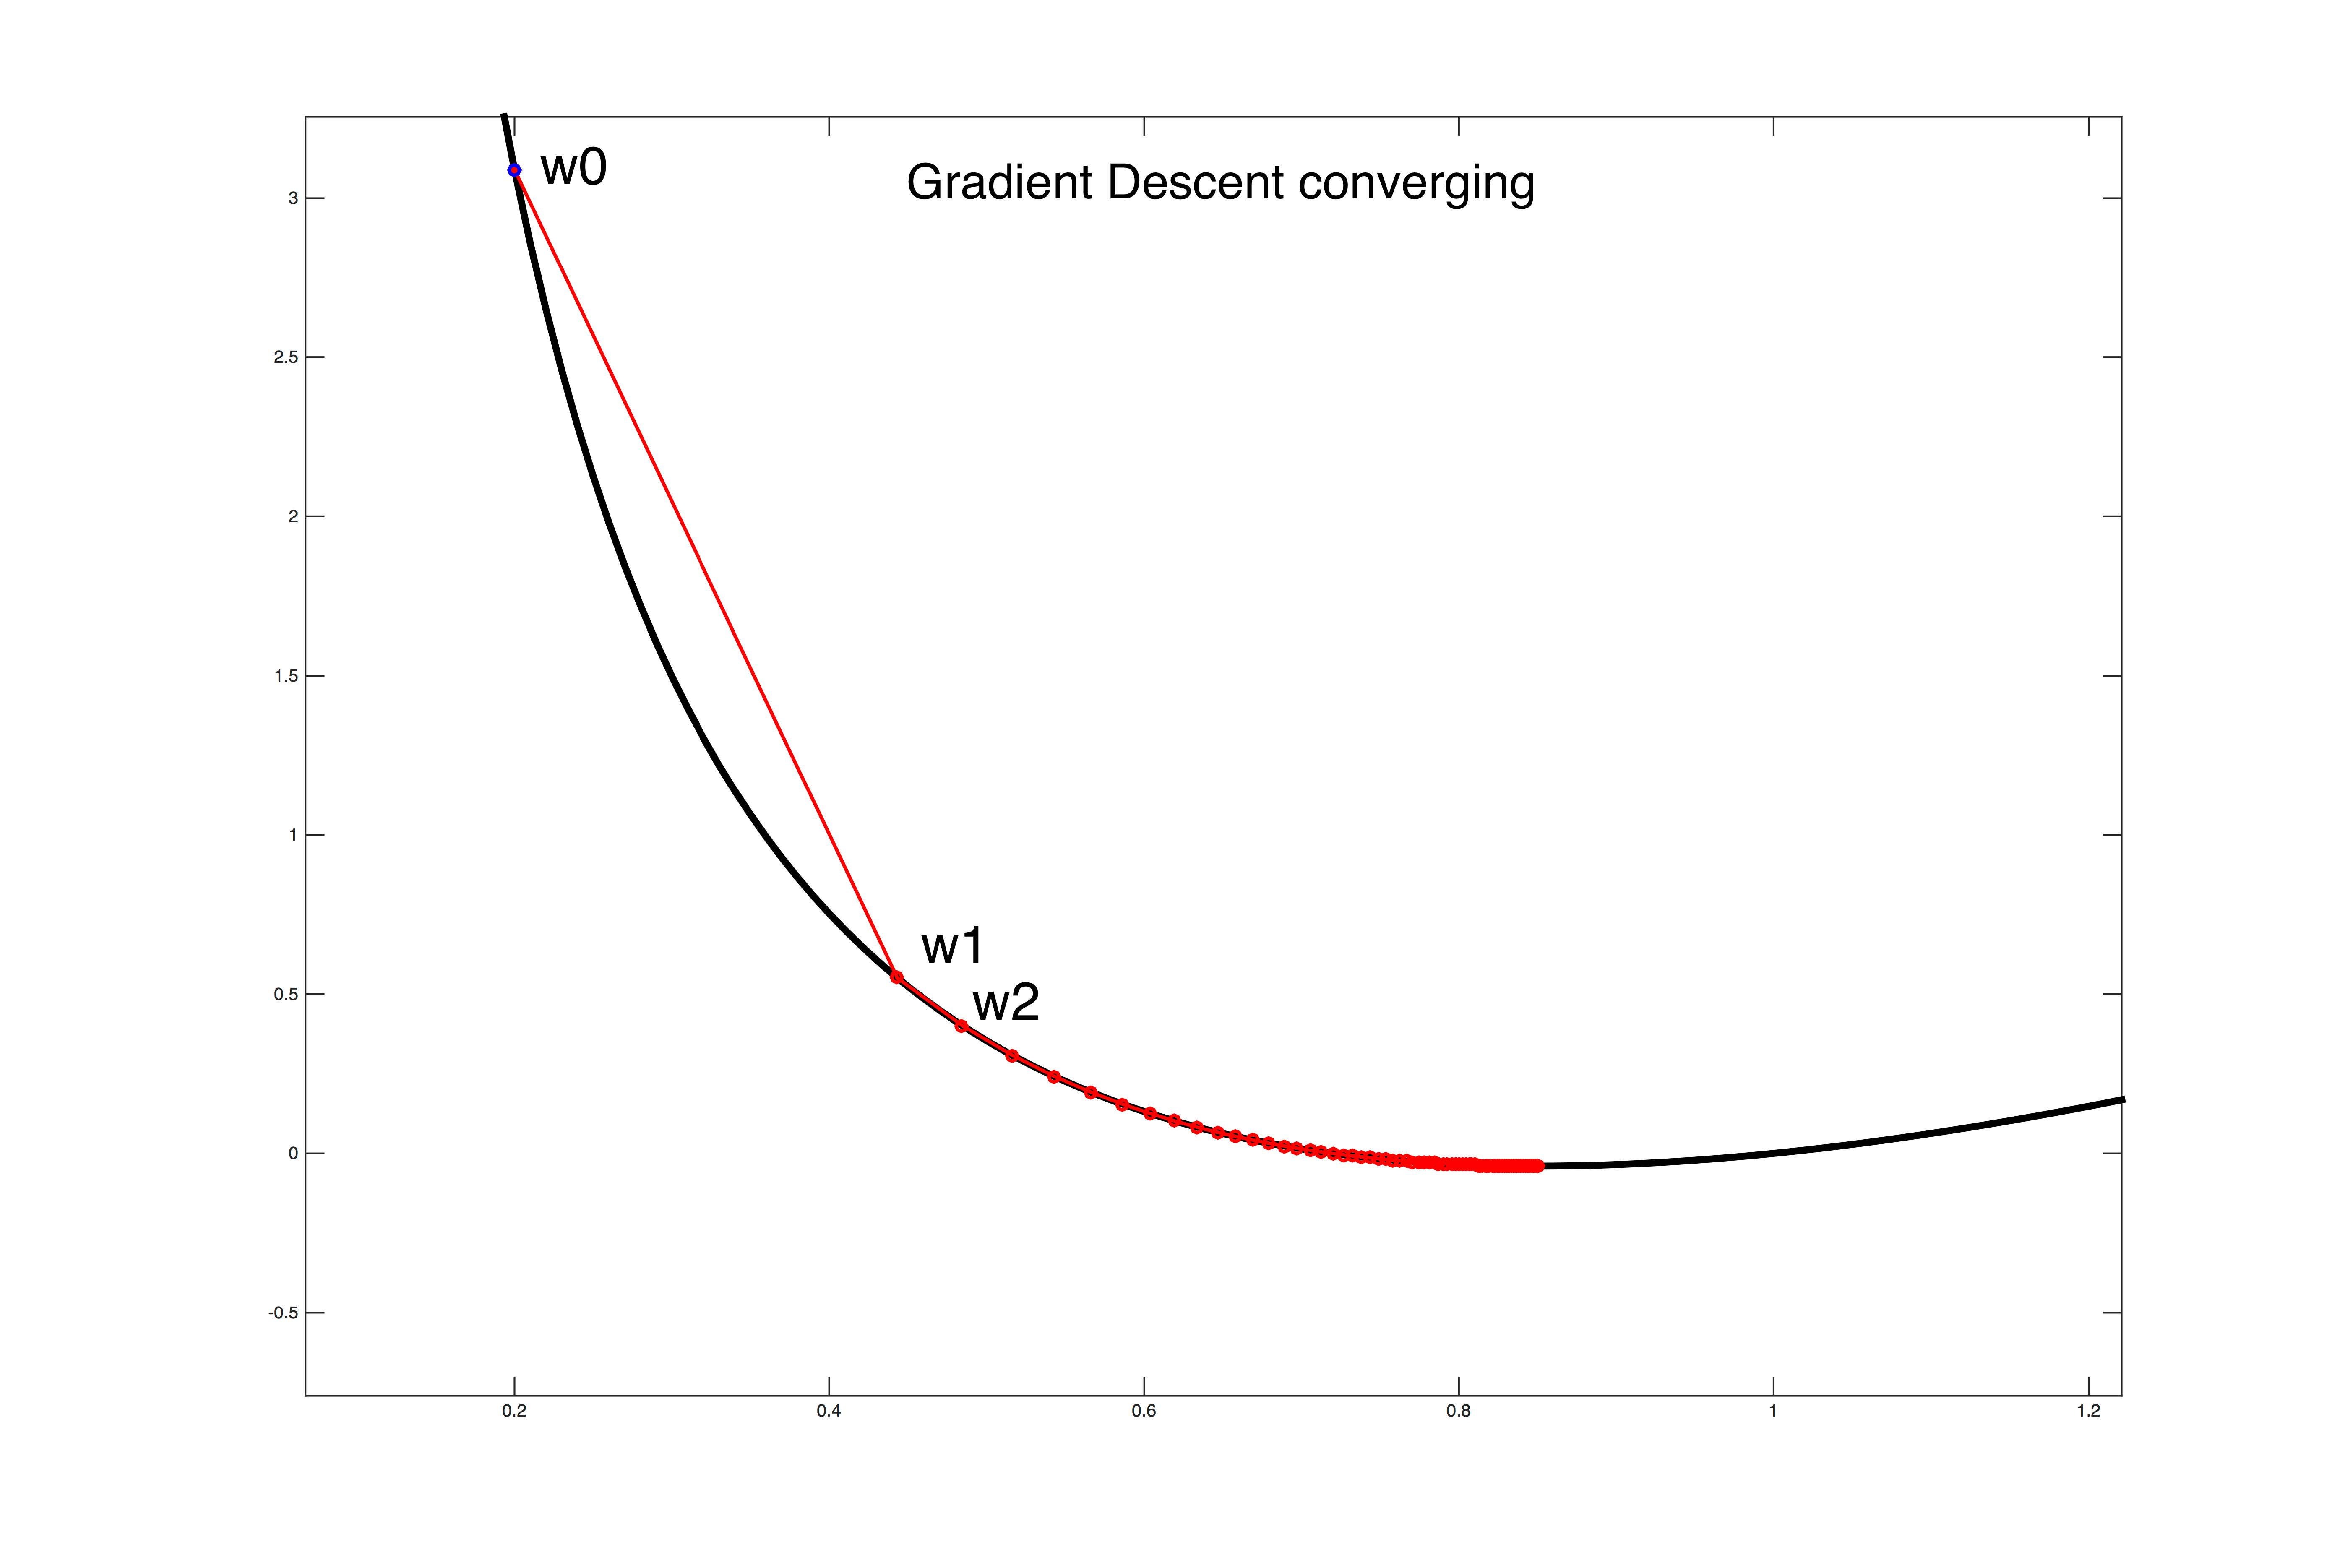
\includegraphics[width=0.55\textwidth]{linear_31.jpg}
		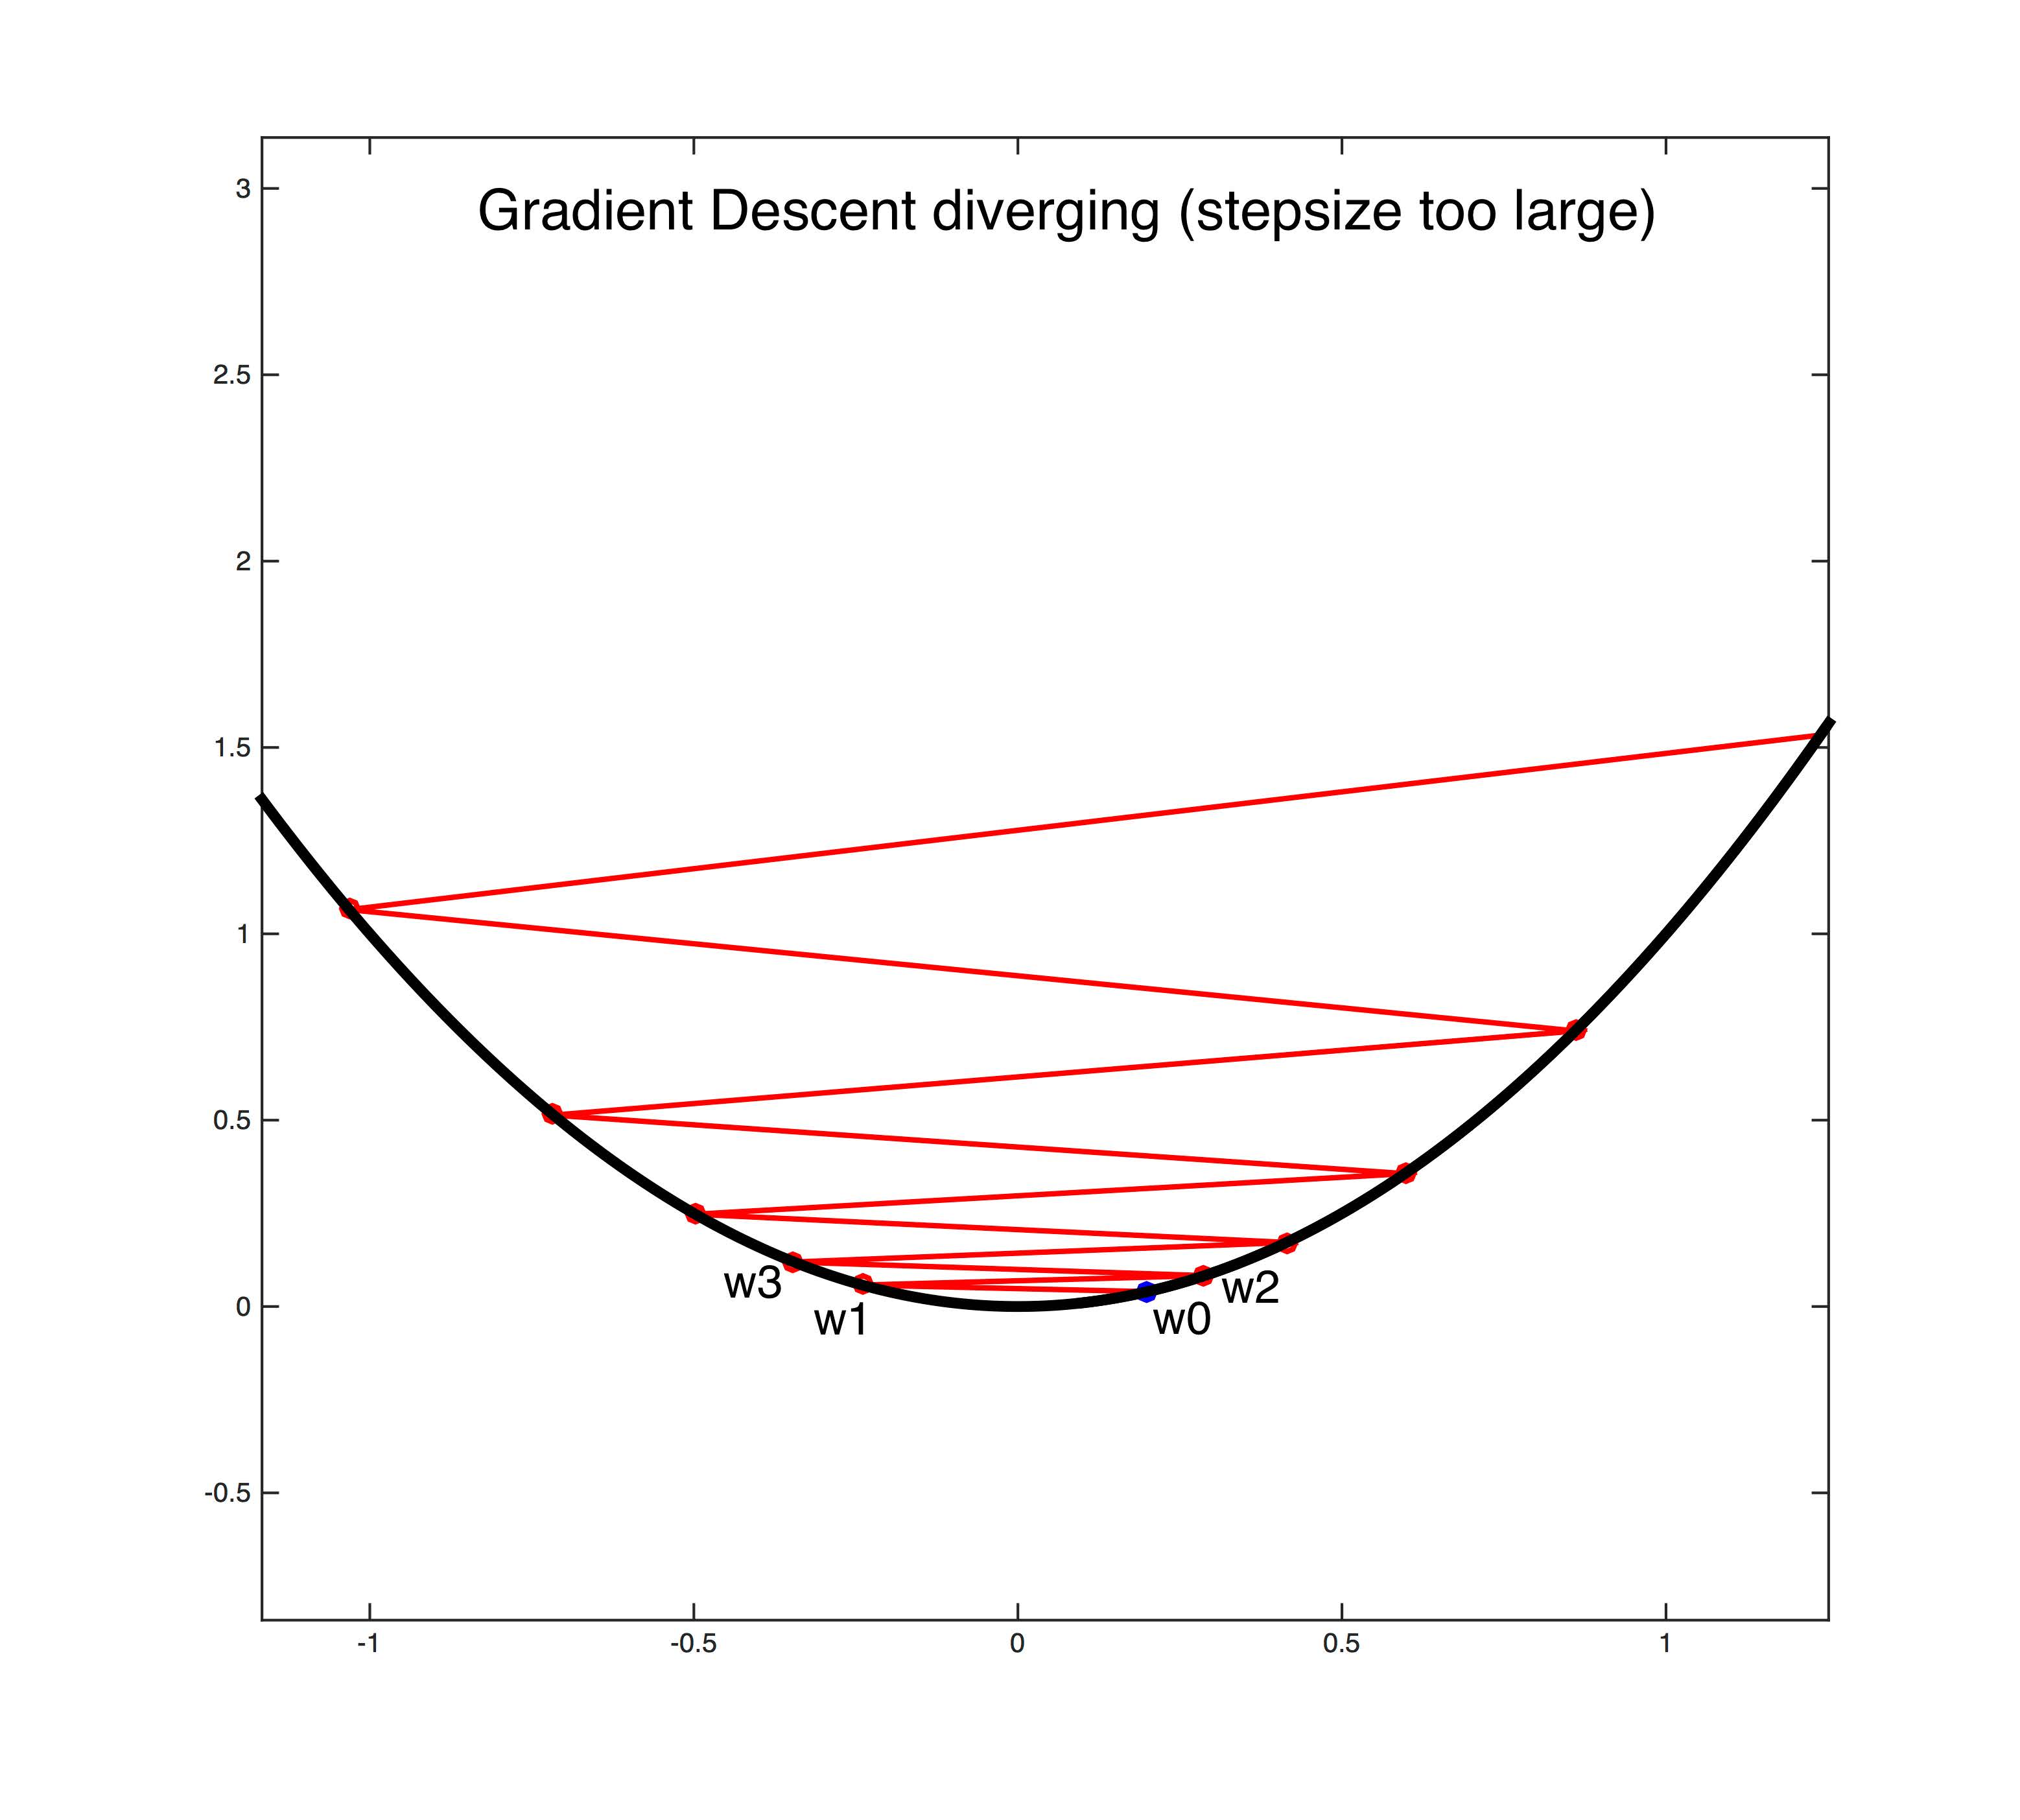
\includegraphics[width=0.4\textwidth]{linear_32.jpg}
	\end{frame}

	\begin{frame}	
		\frametitle{Size of step}
		
		\Large
		\begin{itemize}
			\item Small step - more chance of convergence, but required more iterations
			\item Big step - there is a risk of lack of convergence
			\item Steepest gradient descent:
				\[
					\eta_t = arg\min_\eta Q(w^{t-1}-\eta \nabla Q(w^{t-1})
				\]
			\item It is necessary to do a one-dimensional search at each iteration
		\end{itemize}

	\end{frame}

	\begin{frame}	
		\frametitle{Size of step}
		
		\begin{columns}
			\begin{column}{0.5\textwidth}
				\begin{itemize}
					\item Usually use heuristics
					\item The closer to a minimum, the less it is necessary to tread
					\item Works well
					\[
						\eta_t=\frac{1}{t}
					\]
					\item Even better: $\eta_t=\lambda\left( \frac{s}{s+t} \right)^p$
				\end{itemize}
			\end{column}
			\begin{column}{0.5\textwidth}
				\centering
				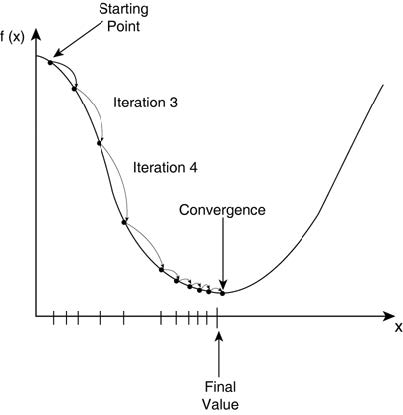
\includegraphics[width=0.9\textwidth]{linear_33.jpg}
			\end{column}
		\end{columns}
		
	\end{frame}

	\begin{frame}	
		\frametitle{Other optimization methods}
		
		\Large
		\begin{itemize}
			\item First-order methods - use first derivatives
			\begin{itemize}
				\item Gradient descent
				\item Stochastic gradient descent
				\item Quasi-Newtonian methods, BFGS
				\item Stochastic Average Gradient, Nesterov momentum, ...
				
			\end{itemize}
			\item Second-order methods - use second derivatives
			\begin{itemize}
				\item The Newton method
			\end{itemize}
			\item Zero-order methods - without derivatives
			\begin{itemize}
				\item Coordinate descent
				\item Stochastic optimization
			\end{itemize}
			
		\end{itemize}
		
	\end{frame}

	\section{Nuances}
	\subsection{5.1}
	\begin{frame}	
		\frametitle{Nuances in learning linear regressors}
		
		\Large
		\begin{itemize}
			\item Selecting the step length $\eta$ - we try different values
			\item The sample must be scaled
			\item Features should not be correlated
		\end{itemize}

	\end{frame}

	\begin{frame}	
		\frametitle{An example}
		
		\Large
		\[
			X = \begin{pmatrix}
				1 & 1000 & 5 & 3 & 4 \\
				9 & 9000 & 10 & 5 & 7.5 \\
				5 & 5000 & 1 & 3 & 2
			\end{pmatrix}
		\]
		\begin{itemize}
			\item The task of predicting the profit of the store in the next month
			\item Consider vectors of the matrix (features) as vectors
		\end{itemize}
		
	\end{frame}

	\begin{frame}	
		\frametitle{An example}
		
		\Large
		\[
		X = \begin{pmatrix}
		1 & 1000 & 5 & 3 & 4 \\
		9 & 9000 & 10 & 5 & 7.5 \\
		5 & 5000 & 1 & 3 & 2
		\end{pmatrix}
		\]
		\begin{itemize}
			\item The first and second signs:$x_2 = 1000x_1$
			\item First - the total weight of goods in tonnes, the second - in kilograms
			\item $x_5=0.5x_3+0.5x_4$
			\item Fifth - average profit for the last two months
			\item Third and fourth - profit in the past and the year before last
		\end{itemize}
		
	\end{frame}

	\begin{frame}	
		\frametitle{Linear dependence}
		
		\Large
		Linear dependence - one of the vectors is equal to the sum of the weights of the remaining vectors
		\begin{itemize}
			\item Redundant information
			\item Extra storage costs
			\item Damages some machine learning methods
		\end{itemize}
		
	\end{frame}

	\begin{frame}	
		\frametitle{Linear dependence}
		
		\Large
		\begin{itemize}
			\item Suppose we found a solution $w^*$
			\item Modify: $w_1=w^*+t\alpha$, where $t$ - a number such that:
			
			\[
				\alpha_1x_1+\dots+\alpha_dx_d=\langle \alpha,x\rangle=0
			\]
			\item The worst case is linearly dependent features
			\item The answer of the new algorithm on any object:
			\[
				\langle w_1, x\rangle = \langle w^*+t\alpha,x\rangle=\langle w^*,x\rangle+t\langle \alpha,x\rangle=\langle w^*,x\rangle
			\]
			\item $w_1$ is also s solution!
		\end{itemize}
		
	\end{frame}

	\begin{frame}	
		\frametitle{Correlating features}
		
		\begin{itemize}
			\item Also bad!
		\end{itemize}
		\[
			\rho(\xi \eta)=\frac{\mathbb E(\xi-\mathbb{\xi})(\eta-\mathbb E \eta)}{\sqrt{\mathbb D\xi\mathbb D\eta}}
		\]
		
		\[
			\rho(x, z)=\frac{\sum_{i=1}^l(x_i-\bar x)(z_i-\bar z)}{\sqrt{\sum_{i=1}^l(x_i-\bar x)^2\sum_{i=1}^l(z_i-\bar z)^2}}
		\]
		
		\[
			\bar x = \frac{1}{l}\sum_{j=1}^lx_j, \bar z = \frac{1}{l}\sum_{j=1}^lz_j
		\]
		\begin{itemize}
			\item $\rho(x,z)\in [-1,+1]$
			\item Very roughly: the closer to +1 or -1, the more accurately equation
			\[
				z=az+b
			\]
			\item The measure of linear dependence
		\end{itemize}
	\end{frame}

	\begin{frame}	
		\frametitle{Examples}
		
		\centering
		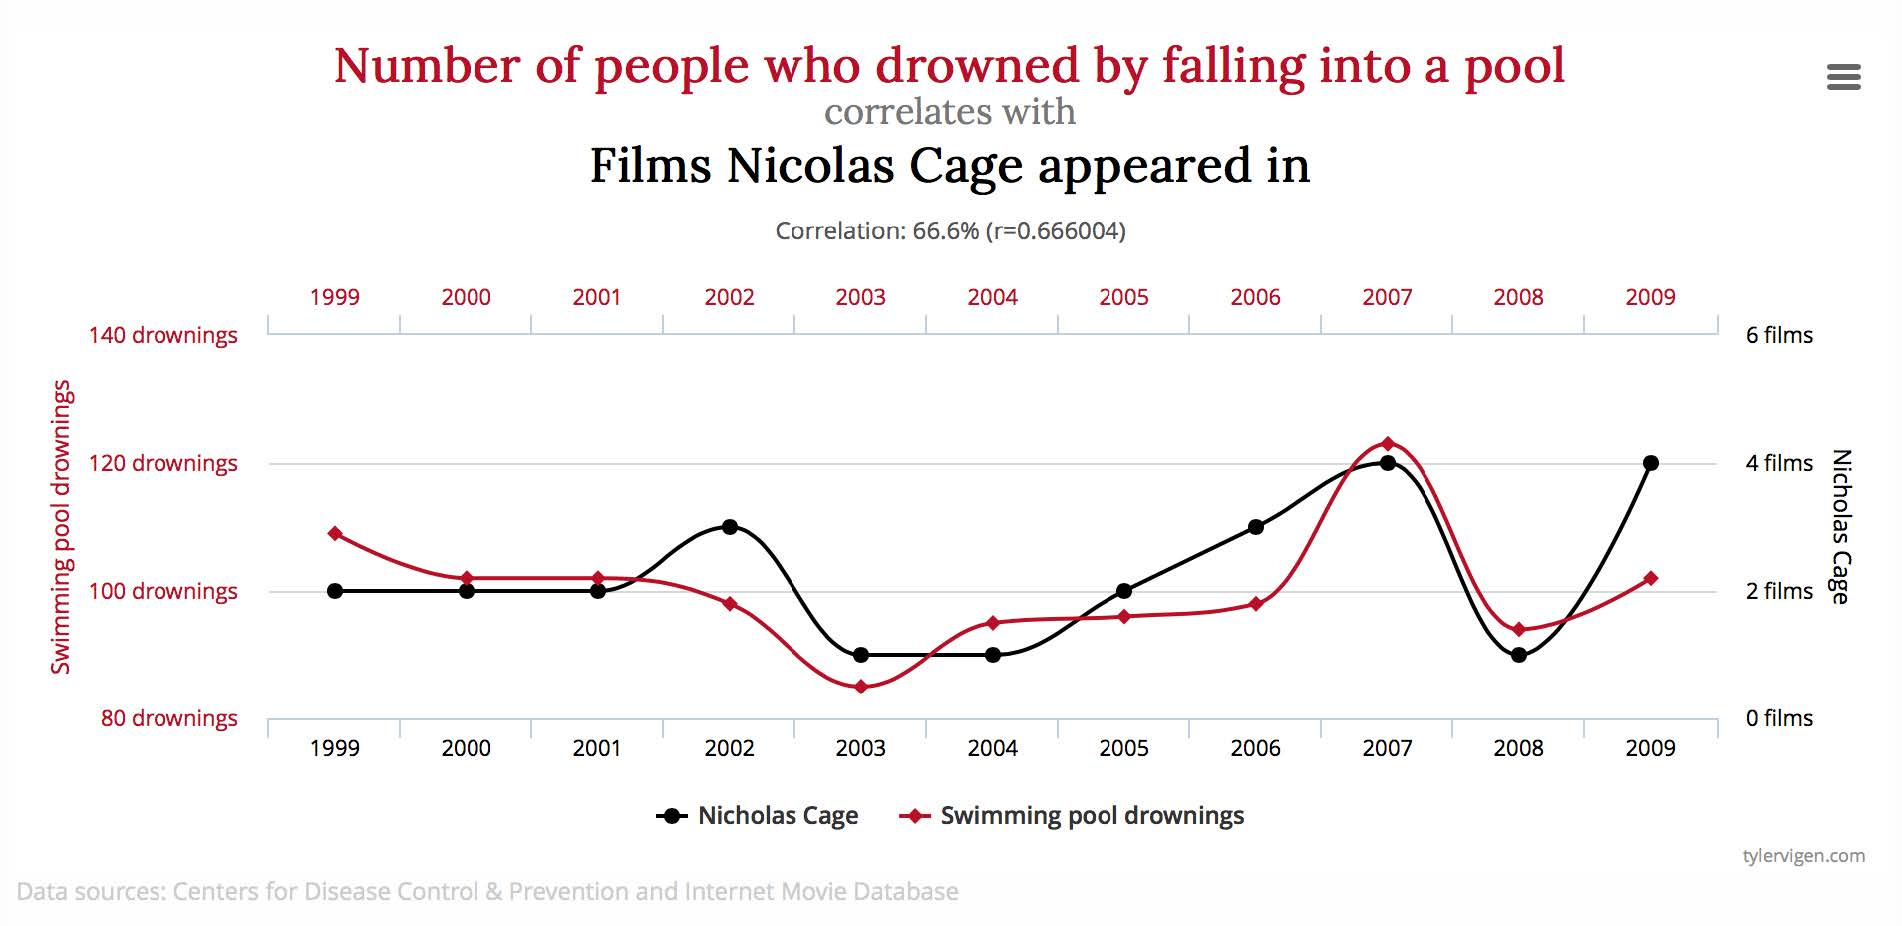
\includegraphics[width=0.9\textwidth]{linear_34.jpg}
	\end{frame}

	\begin{frame}	
		\frametitle{Examples}
		
		\centering
		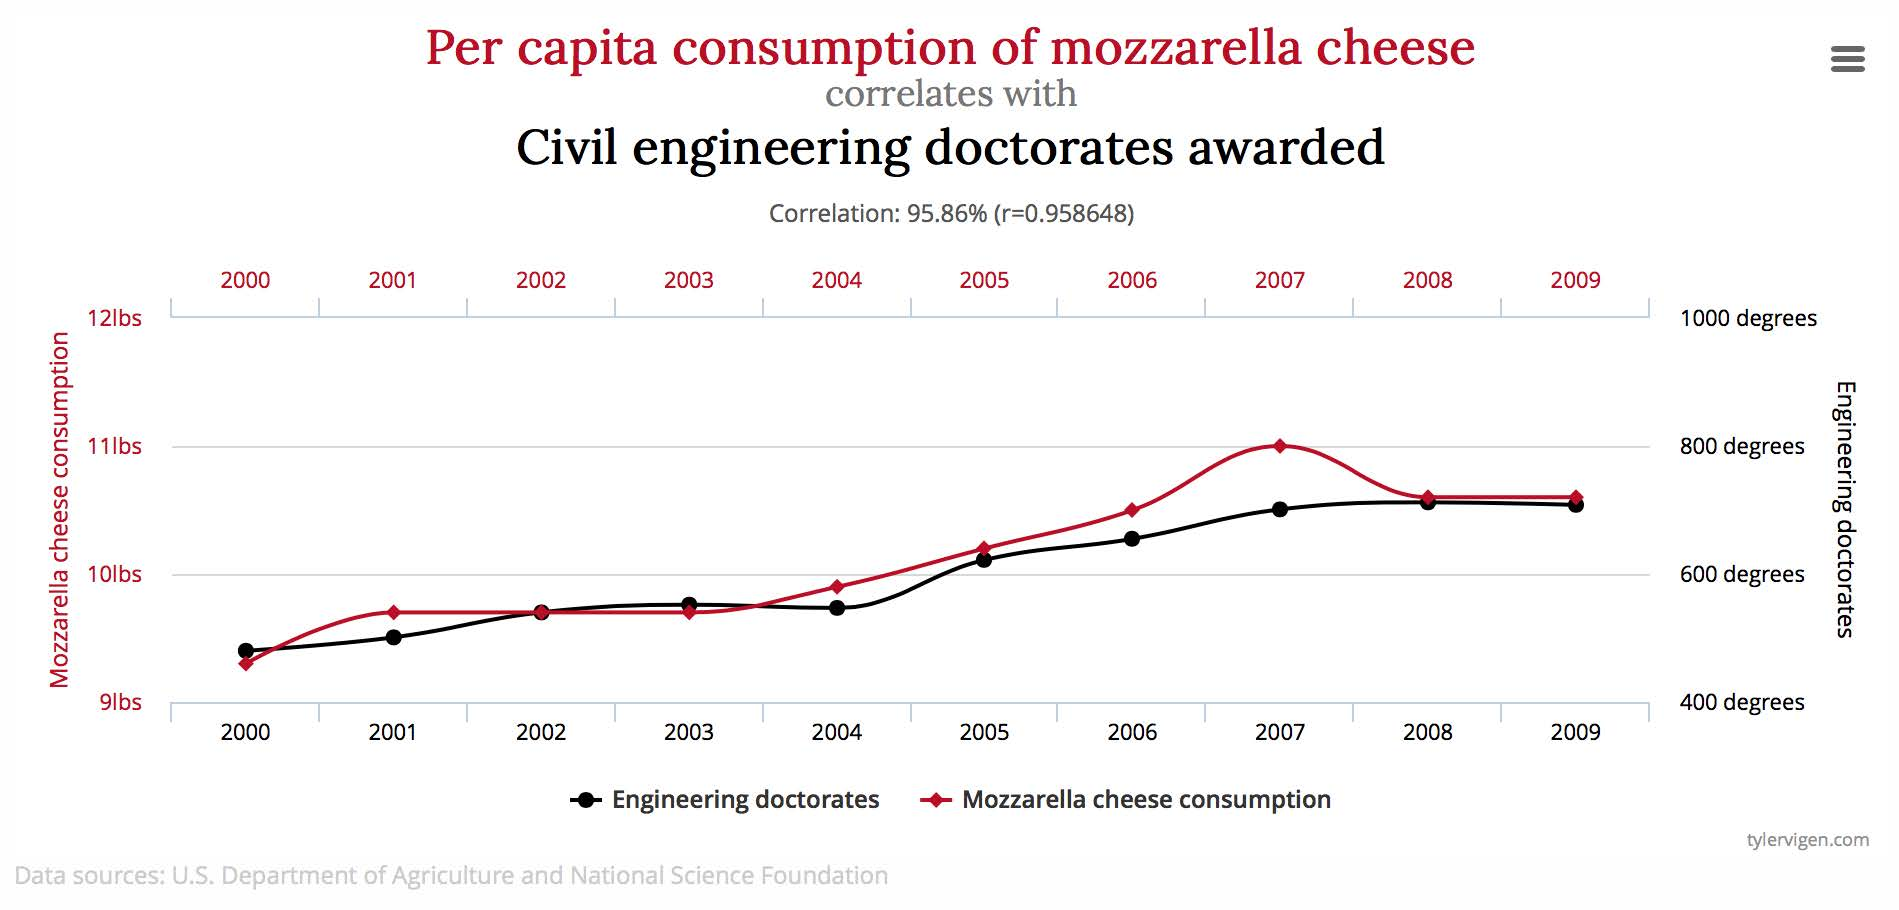
\includegraphics[width=0.9\textwidth]{linear_35.jpg}
	\end{frame}

	\begin{frame}	
		\frametitle{A common misconception}
		
		\Large
		\begin{itemize}
			\item It may seem that correlation follows a causal relationship
			\item This is not true!
			\item Correlation means that events often occur together
			\item But they do not follow each other in any way
			\item More examples: \url{http://tylervigen.com/spurious-correlations} 
		\end{itemize}
		
	\end{frame}

	\begin{frame}	
		\frametitle{Correlating features}
		
		\Large
		\begin{itemize}
			\item It is bad if there are correlating signs
			\item Solution: selection of features or decorrelation
		\end{itemize}
		
		\centering
		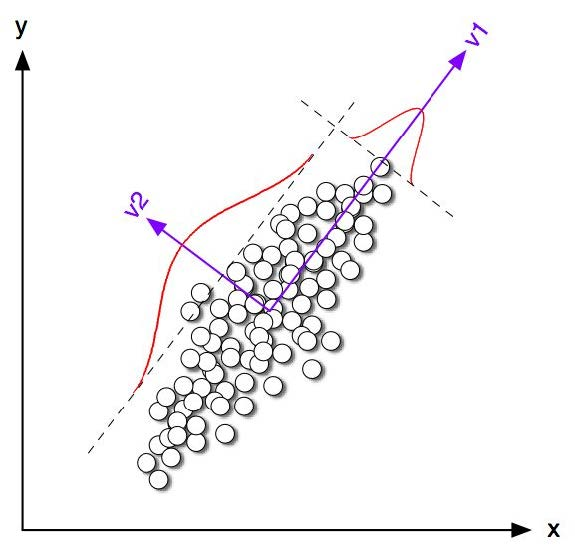
\includegraphics[width=0.6\textwidth]{linear_36.jpg}
	\end{frame}

	\begin{frame}	
		\frametitle{Correlating features}
		
		\begin{itemize}
			\item One feature $x$
			\item $a(x)=w_0+w_1x+w_2x^2+\dots+w9x^9$
		\end{itemize}
		
		\centering
		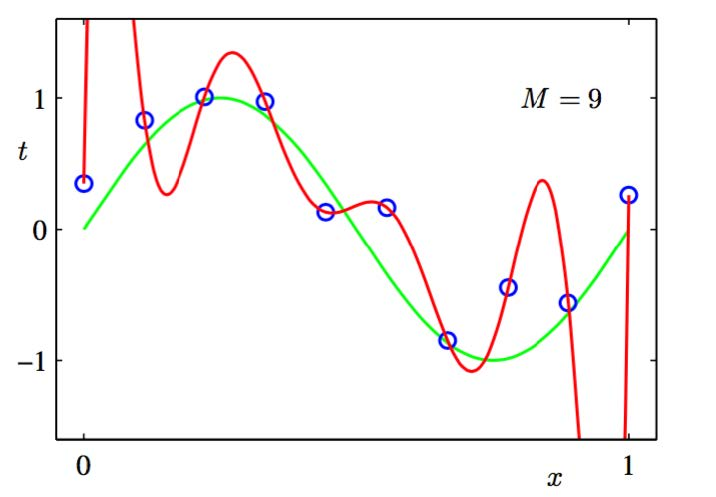
\includegraphics[width=0.5\textwidth]{linear_37.jpg}
		\begin{itemize}
			\item Coefficients:
			\[
				a(x)=0.5+13458922 x - 43983740 x^2 + \dots+ 2740 x^9
			\]
			\item Large coefficients - a symptom of retraining (empirical observation)
		\end{itemize}
	\end{frame}


	\begin{frame}	
		\frametitle{Regularization}
		
		\begin{itemize}
			\item We will fine for the big weights!
			\item Functionality:
			\[
				Q(w,x)=\frac{1}{l}\sum_{i=1}^l (\langle w,x_i\rangle-y_i)^2\rightarrow\min_w
			\]
			\item Regularizer:
			\[
				\|w\|^2=\sum_{j=1}^d w_j^2
			\]
			\item The regularized error functional:
			\[
				\frac{1}{l}\sum_{i=1}^l (\langle w,x_i\rangle-y_i)^2+\lambda \|w\|^2\rightarrow\min_w
			\]
			\item Still smooth and convex
		\end{itemize}
	\end{frame}


	\begin{frame}	
		\frametitle{Regularization}
		\Large
		\begin{itemize}
			\item $\lambda$ - new parameter, it is necessary to select
			\item High $\lambda$  - simple models
			\item Low $\lambda$ - risk of retraining
			\item It is necessary to balance
			\item Selection of $\lambda$ - using cross-validation
		\end{itemize}
	\end{frame}


	\begin{frame}	
		\frametitle{The meaning of regularization}
		\Large
		\begin{itemize}
			\item Minimization of a regularized functional is equivalent to solving a conditional problem:
			\[
				\begin{cases}
					\frac{1}{l}\sum_{i=1}^l (\langle w,x_i\rangle-y_i)^2+\lambda \|w\|^2\rightarrow\min_w\\
					\|w\|^2\leq C
				\end{cases}
			\]
		\end{itemize}
	\end{frame}

	\begin{frame}	
		\frametitle{$L_1$ regularization}
		\Large
		\begin{itemize}
			\item $L_1$ regularizer:
			\[
				\|w\|_1=\sum_{j=1}^d |w_j|
			\]
			\item The regularized error functional:
			\[
			\frac{1}{l}\sum_{i=1}^l (\langle w,x_i\rangle-y_i)^2+\lambda \|w\|_1\rightarrow\min_w
			\]
			\item Functionality becomes non-smooth
			\item It is more difficult to optimize
			\item But the selection of characteristics
			\item Some of the weights in the solution will be zero
		\end{itemize}
	\end{frame}

	\begin{frame}	
		\frametitle{Scaling the sample}
		
		\centering
		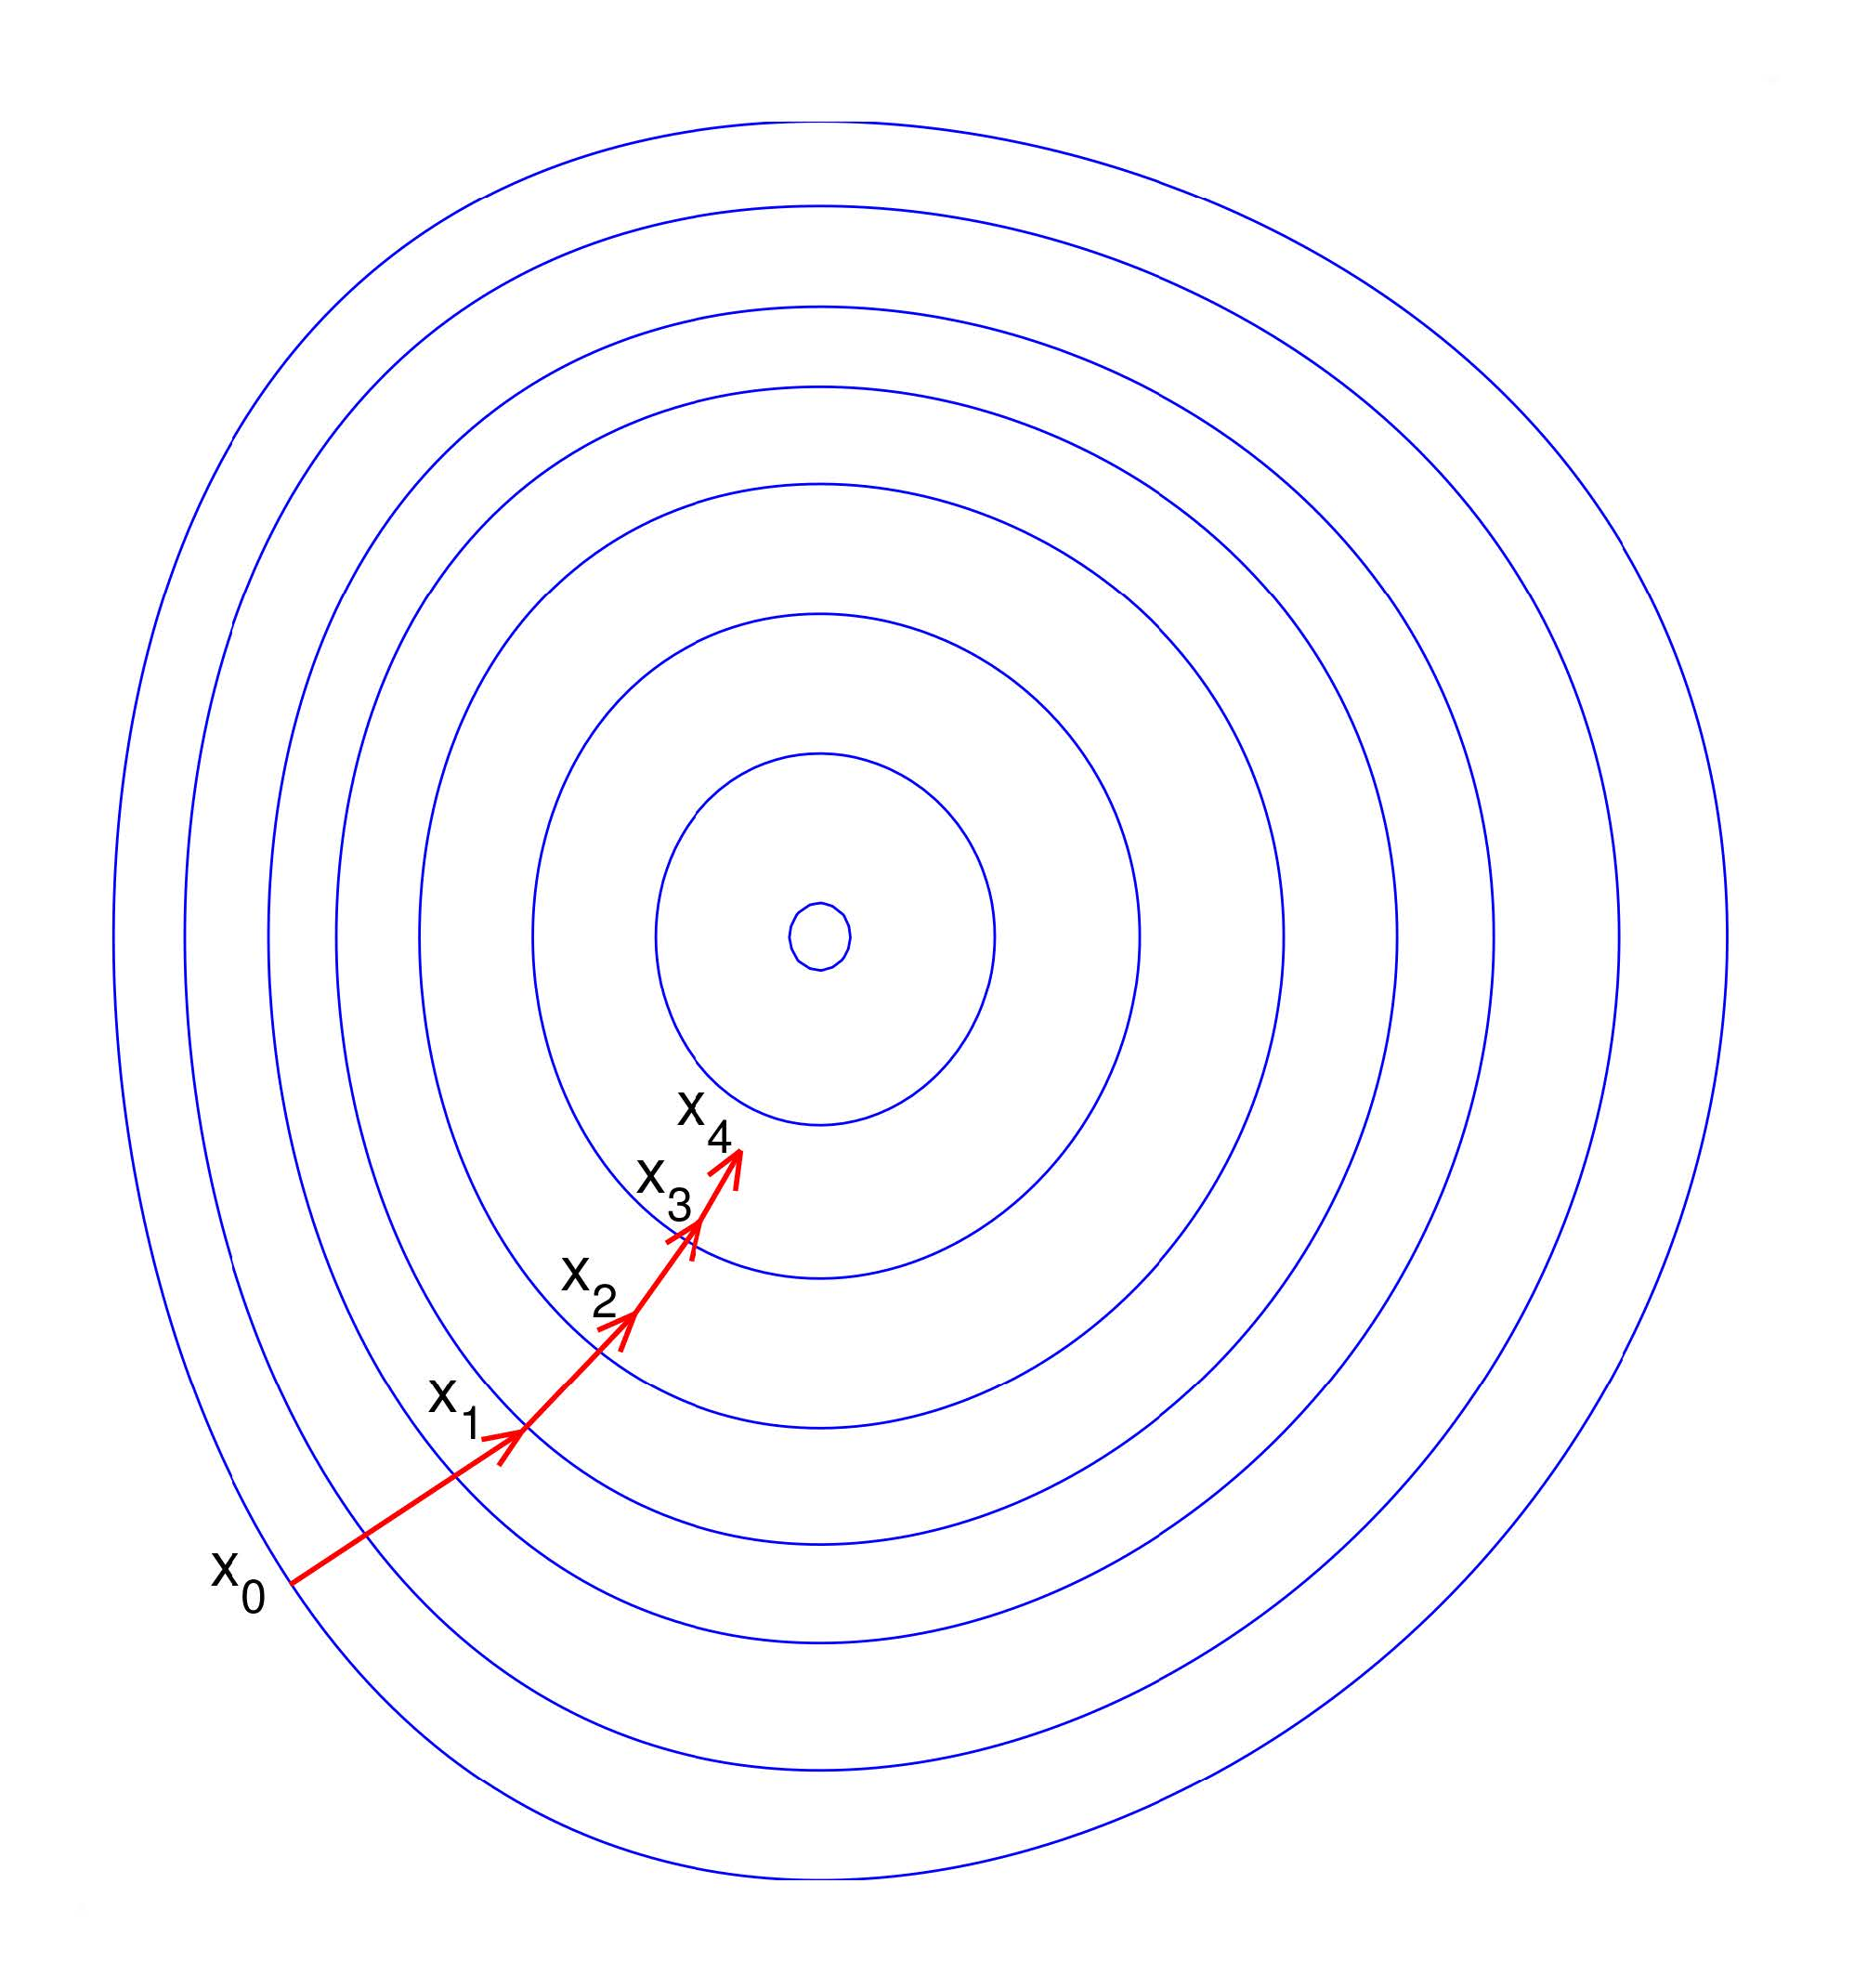
\includegraphics[width=0.45\textwidth]{linear_21.jpg}
		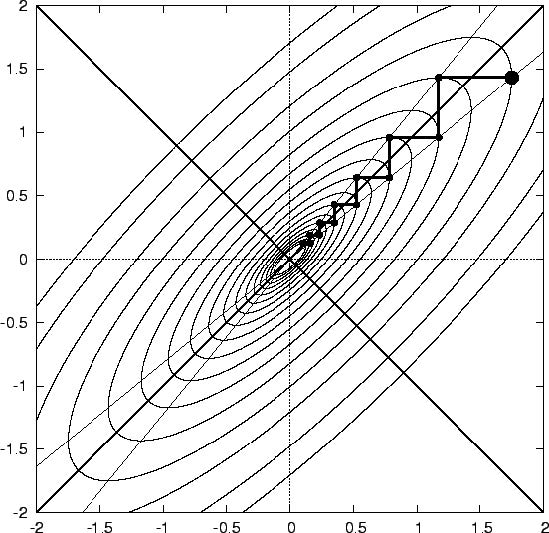
\includegraphics[width=0.45\textwidth]{linear_38.jpg}
	\end{frame}

	\begin{frame}	
		\frametitle{Scaling the sample}
		
		\begin{itemize}
			\item Task: Will the grant application be approved?
			\item 1st feature: how many successful applications did the applicant have before
			\item 2nd feature: the year of birth of the applicant
			\item Scale: units and thousands
			\item All features must have the same scale
		\end{itemize}
	\end{frame}

	\begin{frame}	
		\frametitle{Scaling the sample}
		
		\begin{itemize}
			\item We scale the $j$-th feature
			\item Calculate the mean and standard deviation of the trait on the training sample:
			\[
				\mu_j=\frac{1}{l}\sum_{i=1}^lx_j^j
			\]
			
			\[
				\sigma_j=\sqrt{\frac{1}{l}\sum_{i=1}^l(x_j^j-\mu_j)^2}
			\]		
			\item We scale the $j$-th feature
			\item Subtract from each characteristic value the average and divide by the standard deviation:	
			\[
				x_i^j:=\frac{x_i^j-\mu_j}{\sigma_j}
			\]
		\end{itemize}
	\end{frame}

\end{document}
	
	
